% \PassOptionsToPackage{dvipsnames}{xcolor}

% \documentclass[12pt]{spieman}
% % \documentclass[ACS,STIX1COL]{WileyNJD-v2}
% \usepackage{moreverb}
% \usepackage{graphicx} % Required for inserting images
% \usepackage{xcolor}
% % \usepackage{hyperref}
% \definecolor{MyGreen}{RGB}{141,208,138}
% \definecolor{MyBlue}{RGB}{134,190,220}
% \definecolor{MyOrange}{RGB}{252,128,96}
% \definecolor{MyPurple}{RGB}{174,173,211}

% \usepackage{amsmath,amsfonts,amssymb}
% \usepackage{setspace}
% \usepackage{tocloft}
% \usepackage{amsmath}
% \usepackage{multirow}
% \usepackage{placeins}
% \usepackage{subcaption}
% % \captionsetup[figure]{labelfont=normalsize}

% % \articletype{article}

% \graphicspath{ {./Figures/} }

\chapter[Application of a two-layer skin tissue model]{Application of a two-layer skin tissue model to simulated and experimental data}\label{chap:2layer}

\begin{center}
\begin{minipage}[b]{0.9\linewidth}
\small
\textbf{Foreword\,}
This chapter is an \emph{in extenso} reproduction of \textcolor{red}{cite 2-layer paper here} and has been submitted to Journal of Biomedical Optics for publication. 
\newline
AB has conducted all of the research presented in this chapter under the supervision of JS, MB, and TV. 
\end{minipage}
\end{center}

\minitoc
% \author[1,*]{Anisha Bahl}
% \author[1,3]{Jonathan Shapey}
% \author[2]{Mads Bergholt}
% \author[1]{Tom Vercauteren}
% \affil[1]{School of Biomedical Engineering \& Imaging Sciences, King's College London, 1 Lambeth Palace Road, London, United Kingdom}
% \affil[2]{Department of Craniofacial Development and Stem Cell Biology, King's College London, Guy's Tower, Great Maze Pond, London, United Kingdom}
% \affil[3]{King's College Hospital, Denmark Hill, London, United Kingdom}

% \renewcommand{\cftdotsep}{\cftnodots}
% \cftpagenumbersoff{figure}
% \cftpagenumbersoff{table} 

% \begin{document}
% \maketitle
% \abstract{A two layer model (Yudovsky 2009) is evaluated against Monte Carlo simulations and used to analyse a NIST skin reflectance dataset. To quantify the goodness of fit of this model against simulated reflectance spectra with known ground truth, the normalised root mean squared error is calculated and the mean found to be 0.167 or 0.0402 for quantitative or relative data respectively. When fitted by least squares, the parameter recovery is quantified using linear regression. By focussing on the quality of the oxygen saturation ($StO_2$) recovery, the performance of this model is evaluated across the parameter range and a significant region of failure identified. This failure region corresponds to circumstances where the epidermal layer has significant thickness and melanin content, while the dermal layer has low fraction of blood meaning that the haemoglobin impact is “masked”. The extraction of parameters from the NIST skin dataset using this model returns values that do not correspond well to literature values suggesting that, perhaps, many of these spectra lie within a failure region. This suggests that there are circumstances in which this model performs well, however it should be applied with caution due to its clear regions of failure which limit its use.}
% \keywords{Biological models; Oxygen saturation; Monte Carlo simulations}

% {\noindent \footnotesize\textbf{*}Anisha Bahl,  \linkable{anisha.bahl@kcl.ac.uk} }

\section{Introduction}\label{sec:intro2}
The brain has many layered structures, for example the meninges (dura, pia mater, arachnoid) are all thin layer structures which overlay the cortex. As these are often of the scale that can be penetrated by visible light, this structure should be accounted for in an optical model used to analyse visible spectrum HSI data. Since Yudovsky 2009 was shown to be the best performing single layer model in Chapter \ref{chap:1layer}, the double layer model of the same publication\cite{Yudovsky2009} (developed primarily to model skin) is investigated. Skin is a layered biological tissue structure with data obtained using a well-characterised spectroscopic set-up widely available\cite{Cooksey2017}, so this is treated as a better defined use case to evaluate this layered model. 
%Skin tissue oxygenation ($StO_2$) has been suggested to be a useful metric in the diagnosis and management of pressure ulcers \cite{Wong2003, Mishu2014} and radiative dermatitis \cite{Bashkatov2005}, as well as assisting phlebotomy \cite{FouadAref2021}. For these reasons, efforts have been made to non-invasively quantify $StO_2$ using diffuse reflectance spectroscopy. 

%The diffuse reflectance spectrum of a tissue is influenced by the absorbance and scattering properties of the tissue. Scattering  of tissue is largely dominated by collagen \cite{Anderson1981}. Absorbance of tissue is governed by the chromophores present dominated by haemoglobin which can exist in both oxygenated and deoxygenated states\cite{Prahlc}. These two forms of haemoglobin have differences in absorption which influence the diffuse reflectance spectrum and may allow recovery of the tissue $StO_2$\cite{Clancy2020}. 

%Many methods have been used to quantify $StO_2$ from diffuse reflectance spectroscopy, however few model the spectrum per wavelength, and fewer still provide this modelled spectrum for skin which is characterised by a layered structure. A notable example of this is the Yudovsky 2009 \cite{Yudovsky2009a} based on the Kubelka-Munk theory. Whilst this model has been demonstrated with a variety of experimental data\cite{Yudovsky2011a, Yudovsky2011b}, there has not been a clear evaluation of its performance. 

%Yudovsky's model is based on a single-layer model which we have also evaluated alongside two other prominent single-layer tissue models (a modified Beer-Lambert model \cite{Clancy2015}, and a more elaborate Beer-Lambert-based model proposed by Jacques \cite{Jacques1999})\textcolor{red}{Cite one layer paper}. These models are better suited to open surgical cases where the tissue seen can be approximated as a single homogeneous layer. 

Monte Carlo simulations may be used to model both homogeneous and layered tissues interactions with light of a range of wavelengths. Whilst Monte Carlo is a well-established simulation approach, however as in Chapter \ref{chap:1layer} it is highly computationally challenging to apply the inverse model and so optical properties are challenging to extract.

In this chapter we aim to quantify the performance of the two-layer Yudovsky model by evaluating it against simulated data with known ground truth parameters, as well as fitting the two-layer model to experimental data. The evaluation against simulation is quantified in terms of the forward models (utilising ground truth values within the models to predict the diffuse reflectance spectra), and for the inverse problem solving (evaluating the fidelity of the parameter extraction when fitting to the simulated or measured data); whereas evaluation against experimental data is achieved using the inverse model and comparing the extracted parameters to literature values. This enables
a thorough evaluation of the Yudovsky two-layer model to enable informed application to clinical settings. 

\section{Methods}\label{sec:methods2}
% \subsection{Single-layer models}\label{sec:methodtissuemodelsingle}
% Three analytical models are compared in this work: modified Beer-Lambert \cite{Clancy2015}, Jacques 1999 \cite{Jacques1999}, and Yudovsky 2009 \cite{Yudovsky2009a}. Each of these provide analytical models aiming to investigate single-layer, homogeneous, semi-infinite tissue to enable analysis of tissue during surgery. All three models contain hyperparameters to account for the impact of changes in refractive index which are fitted Monte Carlo simulations, where a single set of values is fitted to a dataset of 100 spectra using the ground truth tissue parameter values. \textcolor{red}{CITE 1LAYER PAPER}

% \subsubsection{Common absorption and scattering model}\label{sec:opticproperties}
% All three forward models utilise the wavelength dependent absorption and reduced scattering coefficients ($\mu_a(\lambda)$ and $\mu_s'(\lambda)$) to compute a
% diffuse reflectance spectrum. 
% The reduced scattering coefficient relates the scattering coefficient ($\mu_s(\lambda)$) with tissue anisotropy ($g$) as follows: 
% \begin{equation}
%     \mu_s'(\lambda) = \mu_s(\lambda) \times (1-g)
%     \label{eq:reducedscattering}
% \end{equation}
% For biological tissue, the reduced scattering coefficient can be well approximated using Mie theory \cite{Jacques2013}: 
% \begin{equation}
%     \mu_s'(\lambda) = a(\frac{\lambda}{500})^{-b}
%     \label{eq:Mie}
% \end{equation}
% where $a$ and $b$ are Mie scattering coefficients that range between 8\textrm{$cm^{-1}$} and 70\textrm{$cm^{-1}$}, and 0.1 and 3.3 respectively depending on the tissue microstructure \cite{Jacques2013}. 
% The absorption coefficient of most internal, homogeneous, tissues, including dermis, is dominated by haemoglobin in the visible region (450-650 nm)\cite{JacquesAbs} and can be modelled using the following equation \cite{Yudovsky2009a}: 
% \begin{equation}
% \begin{aligned}
%     & \mu_a(\lambda) = f_{blood}\mu_{a, blood}(\lambda) + (1 - f_{blood})\mu_{a, back}(\lambda) \\
%     & \textrm{where} \\
%     & \mu_{a, blood}(\lambda) = c_{HbT}\frac{\ln(10)}{64500}[StO_2 \epsilon_{HbO_2}(\lambda) + (1 - StO_2)\epsilon_{Hb}(\lambda)] \\
%     & \textrm{and} \\
%     & \mu_{a, back}(\lambda) = 7.84\times10^8 \lambda^{-3.255}
% \end{aligned}
% \label{eq:mua}
% \end{equation}
% Here $StO_2$ refers to oxygen saturation, $c_{HbT}$ refers to the total concentration of haemoglobin in whole blood commonly taken as 150\textrm{$gL^{-1}$}\cite{Prahlb}, with $StO_2$ denoting the fraction of haemoglobin that is oxygenated ($HbO_2$) and the remainder is deoxygenated ($Hb$), and ranges between 0-100\%\cite{Yudovsky2009a}. $f_{blood}$ is the volume fraction of tissue occupied by blood which has absorption coefficient $\mu_{a, blood}(\lambda)$ and typically ranges between 0.2-12\%\cite{Yudovsky2009a}, with the remainder of tissue having background absorption $\mu_{a, back}(\lambda)$\cite{Yudovsky2009a}.
% Finally, $\epsilon_{HbO_2}(\lambda)$ and $\epsilon_{Hb}(\lambda)$ denotes the wavelength-dependent extinction coefficients of the chromophores $HbO_2$ and $Hb$ which are found in the literature\cite{Prahlb}. 

% \subsubsection{Modified Beer-Lambert}
% The modified Beer-Lambert models absorption ($A(\lambda)$) and diffuse reflectance ($R(\lambda)$) as follows: 
% \begin{equation}
% \begin{aligned}
%     & A(\lambda) = L\mu_a(\lambda) + \mu_s'(\lambda) \\
%     & R(\lambda) = \exp{\left(-\frac{A(\lambda)}{100}\right)}
% \end{aligned}
% \label{eq:modBL1}
% \end{equation}
% A factor of 100 is included to convert $\mu_a(\lambda)$ and $\mu_s'(\lambda)$ from the conventional units of cm\textrm{$^{-1}$} to mm\textrm{$^{-1}$}. $L$ describes a differential path length to account for the variety of photon path lengths through scattering media. To simplify this model, $L$ is often approximated to 1 \cite{Clancy2015} and $\mu_s'(\lambda)$ is often modelled as a wavelength-independent constant\cite{Clancy2015, Ma2016}. 
% To allow for improved flexibility in this model,
% we introduce linear scaling hyperparameters ($M_{1-3}$), as shown in Equation \eqref{eq:modBL2}, that are fitted to Monte Carlo simulations at the refractive index of interest. 
% \begin{equation}
% \begin{aligned}
%     & A(\lambda) = M_1\mu_a(\lambda) + M_2\mu_s'(\lambda) + M_3 \\
%     & R(\lambda) = \exp{\left(-\frac{A(\lambda)}{100}\right)}
% \end{aligned}
% \label{eq:modBL2}
% \end{equation}

% \subsubsection{Jacques 1999}
% The Jacques model is also based on the Beer-Lambert model using the assumption that a wavlength-dependent path length $L(\lambda)$ can approximate the ensemble of path lengths experienced by photons in a tissue by $L(\lambda) = A(\lambda)\delta(\lambda)$ where $A(\lambda)$ and $\delta(\lambda)$ are defined in Equation \ref{eq:Jacques}. This results in the following model with the hyperparameters ($M_{1-3}$) which the authors fit to Adding Doubling simulations \cite{Jacques1999}. In our work, we refit these to Monte Carlo simulations since these are considered the gold standard optical simulation method and improve the model fitting results. 
% \begin{equation}
% \begin{aligned}
%     & N'(\lambda) = \frac{\mu_s'(\lambda)}{\mu_a(\lambda)} \\
%     & \delta(\lambda) = \frac{1}{\sqrt{3\mu_a(\lambda)[\mu_a(\lambda) + \mu_s'(\lambda)]}} \\
%     & A(\lambda) = M_1 + M_2\exp \left[ \frac{\ln(N'(\lambda))}{M_3} \right] \\
%     & R(\lambda) = \exp[-A(\lambda)\delta(\lambda)\mu_a(\lambda)] \\
% \end{aligned}
% \label{eq:Jacques}
% \end{equation}

% \subsubsection{Yudovsky 2009}\label{sec:Yudovskysingle}
% \subsection{Double-layer model}\label{sec:methodtissuemodeldouble}
\subsection{Modelling tissues}\label{sec:methodtissuemodeldouble}
\subsubsection{Common absorption and scattering model}\label{sec:opticproperties2}
As described in Chapter \ref{chap:1layer}, the forwards model for each layer utilises the wavelength dependent absorption and reduced scattering coefficients ($\mu_a(\lambda)$ and $\mu_s'(\lambda)$) to compute a diffuse reflectance spectrum. 
The reduced scattering coefficient of both dermis and epidermis is modelled identically to that in Section \ref{sec:opticproperties}. The absorption coefficient of most internal, homogeneous, tissues, including dermis, and so is also modelled identically to that in Section \ref{sec:opticproperties}. When modelling skin, it is necessary to use more than one layer due to the stark differences in optical and anatomical properties between the layers of skin\cite{Mignon2018}. In this chapter each of these layers has a distinct absorption coefficient ($\mu_a(\lambda)$) and identical reduced scattering coefficient ($\mu_s'(\lambda)$). The epidermal $\mu_a(\lambda)$ ($\mu_{a, 1}(\lambda)$) is modelled with the major chromophore melanin, characterised by its volume fraction $f_{mel}$ (ranging between 1-43\% \cite{Yudovsky2009}) and no blood, as described in Equation \ref{eq:muaepi}. 
\begin{equation}
\begin{aligned}
    & \mu_{a, 1}(\lambda) = f_{mel}\mu_{a, mel}(\lambda) + (1-f_{mel})\mu_{a, back}(\lambda) \\
    & \textrm{where}\\
    & \mu_{a, mel}(\lambda) = 6.60\times10^{11}\lambda^{-3.33}\\
    & \textrm{and}\\
    & \mu_{a, back}(\lambda) = 7.84\times10^8\lambda^{-3.255}\\
\end{aligned}
\label{eq:muaepi}
\end{equation}
The dermal $\mu_a(\lambda)$ ($\mu_{a, 2}(\lambda)$) is modelled as dominated by blood, and a single $\mu_s'(\lambda)$ is modelled to characterise both layers, as described in Equation \ref{eq:mua}. As this model is specified to a subset of tissue types associated with skin, the tissue parameters are restricted by Yudovsky to narrower bands of 20-100\% for $StO_2$, 0.2-7\% for $f_{blood}$\cite{Yudovsky2011a} and the scattering tissue parameters are also limited to 30-70cm$^{-1}$ and 0.7-2.5 for $a$ and $b$ respectively to better reflect those of skin\cite{Jacques2013}. 

\subsubsection{Yudovsky 2009 model}\label{sec:Yudovsky2009}
% The original Yudovsky model presents a complex analytical derivation \cite{Yudovsky2009a} of a single-layer reflectance equation for each tissue layer with a simplified formulation subsequently presented in their Erratum \cite{Yudovsky2015}. The model takes the reduced albedo ($w'(\lambda)$), calculated from $\mu_a$ and $\mu_s'$, as input and returns the diffuse reflectance spectra ($R(\lambda)$). This provides an easily applicable model with hyperparameters ($M_{1-6}$) which are quoted for a refractive index ($n$) of 1.44. We found that these can be fitted to Monte Carlo spectra to allow for use with other refractive indices\textcolor{red}{COULD CITE 1LAYER PAPER}. This simplified formulation is used within this work. 
% \begin{equation}
% \begin{aligned}
%     & w'(\lambda) = \frac{\mu_s'(\lambda)}{\mu_a(\lambda) + \mu_s'(\lambda)} \\
%     & R = M_1 + M_2\exp{\left[ M_3w'(\lambda)^{M_4}\right]} + \frac{M_5}{1.02 - M_6} \\
% \end{aligned}
% \label{eq:Yudovskysingle}
% \end{equation} 
% 
The Yudovsky two layer model is a complex interaction between the Yudovsky single layer model, detailed in Section \ref{sec:Yudovskysingle}, applied to two layers\cite{Yudovsky2009}. These two layers represent the epidermis ($1$) and dermis ($2$), where the former has thickness $L_1$ (discussed in \textrm{$\mu m$} but input in $cm$) and the latter is semi-infinite.
These single layer reflectances are then combined as in Equation \ref{eq:Pilondouble} using a reduced reflectance ($R^*$) which is calculated using $L_1$, $w_{tr, 1}$, and $w_{tr,2}$ as in Equation \ref{eq:reducedR}. 
\begin{equation}
\begin{aligned}
    & \xi = \sqrt{\frac{47}{52} + \frac{31}{49}w_{tr, 1} - \frac{49}{54}w_{tr, 1}^2 - \frac{17}{27}w_{tr, 1}^3} \\
    & Y_1 = \xi(\mu_{a,1} + \mu_s')L_1 \\
    & \frac{1}{\alpha} = 2.562 - \frac{4.263}{3.050 - w_{tr, 2}} \\
    & R^* = \frac{\tanh{Y_1}}{\frac{1}{\alpha} + (1 - \frac{1}{\alpha})\tanh{Y_1}} \\
\end{aligned}
\label{eq:reducedR}
\end{equation}
Equation \ref{eq:Pilondouble} returns the diffuse reflectance spectrum, however this can be converted to total reflectance by addition of a constant offset of 0.0325 for a refractive index of 1.44 (for tissues)\cite{Yudovsky2011a}.
\begin{equation}
    R = R^*(R_{s1} - R_{s2}) + R_{s2}
\label{eq:Pilondouble}
\end{equation}
Often in clinical settings it is difficult to obtain precise quantitative data and so relative data is used instead\cite{Bahl2023}. For the purposes of this work, we define relative data to be mean normalised spectra using the mean of all wavelengths below 600nm. 

\subsection{Reference spectra}\label{sec:methodreference2}
Similarly to Section \ref{sec:methodreference}, 100 Monte Carlo simulations are generated by selecting random values for the variables $a$, $b$, $StO_2$, $f_{blood}$, $f_{mel}$, and $L_1$ which are bounded to 30-70cm\textrm{$^{-1}$}, 0.7-2.5, 20-100\%, 0.2-7\%, 1-43\%, and 20-150\textrm{$\mu m$} respectively to represent the range seen in skin \cite{Jacques2013, Yudovsky2009}. These are converted to $\mu_a$ and $\mu_s'$ values as in Section \ref{sec:opticproperties2}. Monte Carlo takes $\mu_a$ and $\mu_s$ as inputs for each layer so a random value of $g$ is chosen per spectrum between 0.7-0.9 to convert $\mu_s'$ to $\mu_s$ using Equation \ref{eq:reducedscattering}. The diffuse reflectance spectra are then generated using CUDAMCML\cite{Alerstam2008} to propagate 10000 photons through a geometry of a slab of thickness $L_1$ of epidermis with optical properties $\mu_{a,1}$ and $\mu_s'$ and a 3cm (to approximate semi-infinite) slab of dermis with optical properties $\mu_{a, 2}$ and $\mu_s'$. When fitting models to these spectra for parameter extraction, the same bounds are imposed on the fitting routine. 

The NIST dataset measured total reflectance from the forearms of 100 healthy volunteers using an integrating sphere spectrophotometer\cite{Cooksey2017}. Three replicates were measured of which we utilise the mean for each volunteer to create the reference set of 100 spectra used for this work. 
\FloatBarrier

\subsection{Evaluation of model performance}\label{sec:methodevaluate2}
This model is evaluated against reference spectra with known ground truth parameters generated using Monte Carlo as detailed in \ref{sec:methodreference2}, and experimental data as provided by a NIST skin dataset\cite{Cooksey2017}, which does not have known ground truth parameters. 

When evaluating against Monte Carlo simulation, both the forwards and the inverse model can be evaluated as in Section \ref{sec:methodevaluate}, where the forwards model is evaluated using $NRMSE$ and the inverse model is evaluated in terms of correlation and $APE$. 
% The similarity of the forwards models ($s$) generated using ground truth parameters compared to the reference spectra ($r$) at all wavelengths ($\lambda$) are quantified using the Normalised Root Mean Squared Error ($NRMSE$), defined in Equation \ref{eq:NRMSE}.
% \begin{equation}
%     NRMSE = \frac{\sqrt{\frac{1}{\Lambda}\sum_{\lambda}^{\Lambda}\left(s_{\lambda} - r_{\lambda}\right)^2}}{\sqrt{\frac{1}{\Lambda}\sum_{\lambda}^{\Lambda} r^2_{\lambda}}}
%     \label{eq:NRMSE}
% \end{equation}

% The model is also evaluated on its ability to recover the ground truth parameters when fitted using a least squares fitting approach (using SciPy v1.10.0 \href{https://docs.scipy.org/doc/scipy/reference/generated/scipy.optimize.least_squares.html}{\texttt{scipy.optimize.least\_squares}} function) to the reference spectra. 
It is noted that this model is not suitable for wavelengths above 600nm \cite{Yudovsky2011a} and therefore a weighting function is used to ensure only wavelengths below 600nm are considered. It is found that increasing the weighting in the region 525-585nm, ie. the region corresponding to the major Haemoglobin peaks, improves the fit. The weighting function used can be seen in Figure \ref{fig:weighting}. 
\begin{figure}
    \centering
    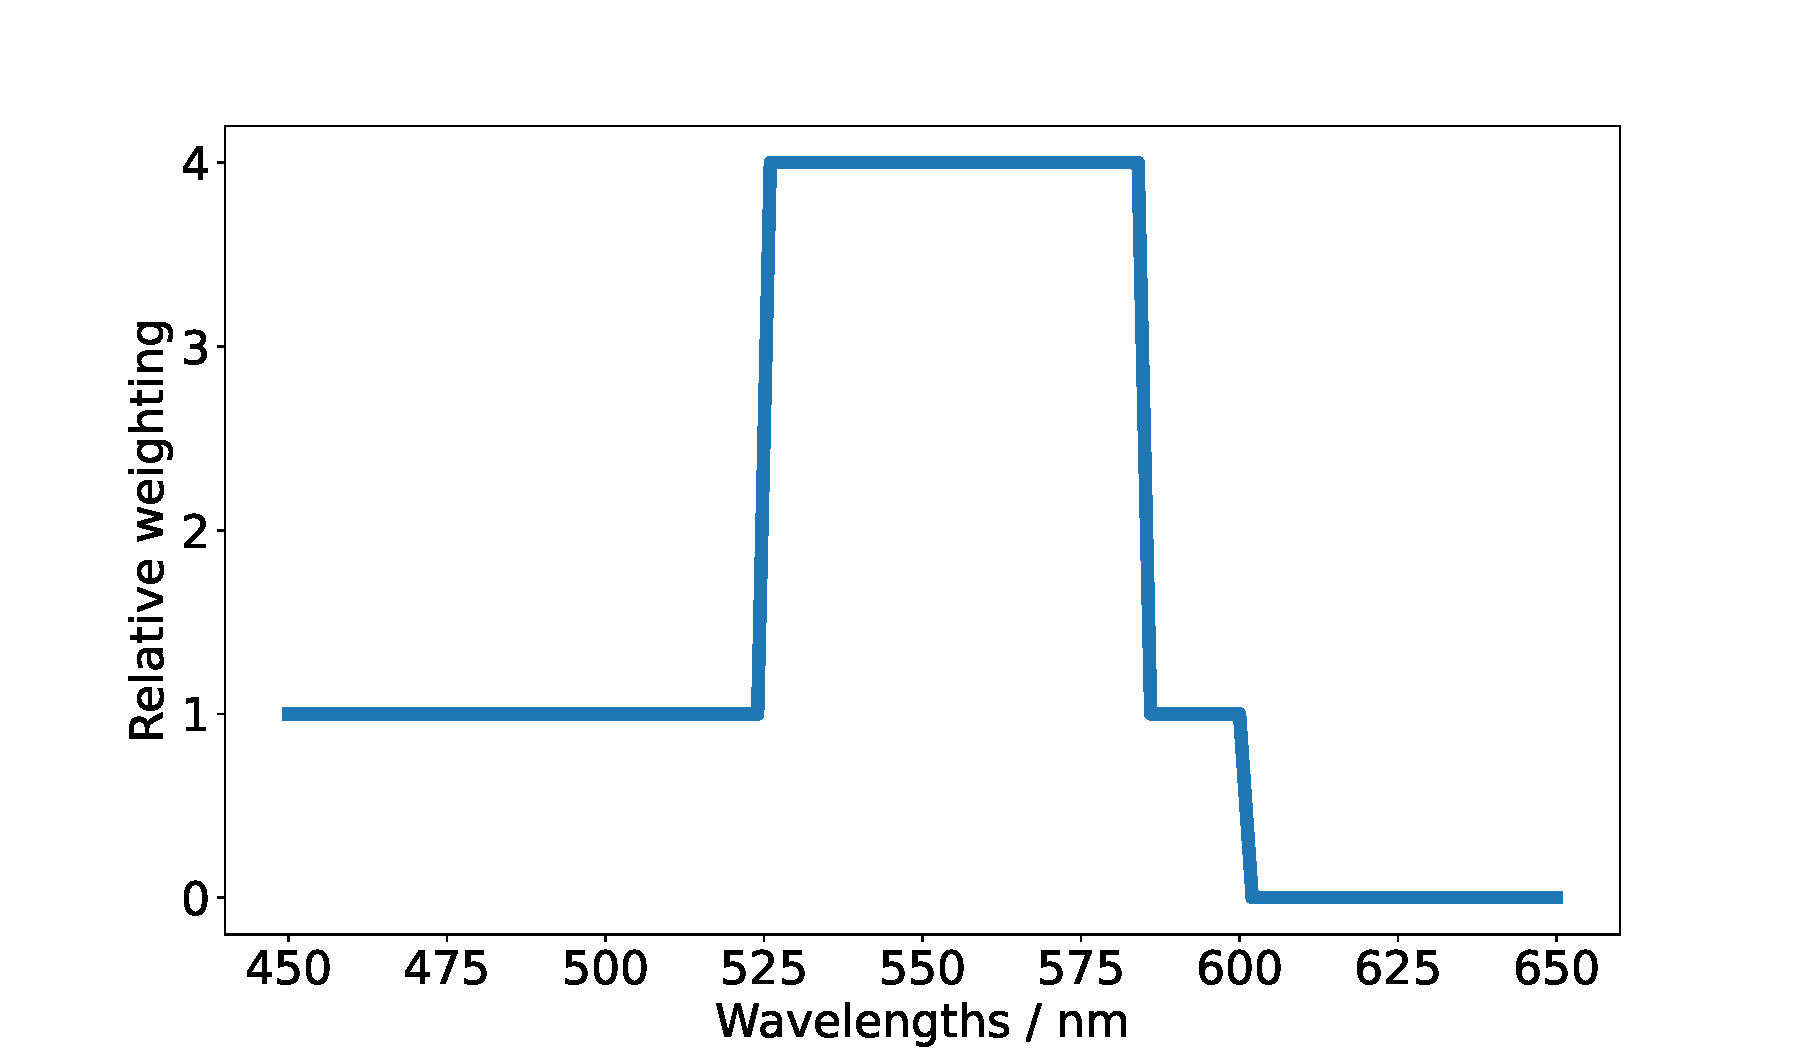
\includegraphics[width=0.6\textwidth]{wavelength_weighting}
    \caption{Relative weighting of wavelengths in residual used for least squares fitting of the two layer Yudovsky model.}
    \label{fig:weighting}
\end{figure}
The correlation between the ground truth and fitted parameters is calculated (using SciPy v1.10.0 \href{https://docs.scipy.org/doc/scipy/reference/generated/scipy.stats.linregress.html}{\texttt{scipy.stats.linregress}} function) and evaluated using the Pearson correlation coefficient ($r$) and the p-value ($p$). We take $p < 0.05$ to demonstrate significance at a 95\% confidence level for a hypothesis test with the null hypothesis that there is no correlation. 

To demonstrate the regions of parameter space where the Yudovsky 2-layer model varies in performance quality, for each combination of absorbance parameters (and one set of scattering parameters) 10 Monte Carlo diffuse reflectance spectra are simulated where the $StO_2$ is varied between 0 and 100\% and scattering parameters are fixed. The Yudovsky two layer model is fitted by least squares to each of these Monte Carlo spectra and a linear regression is fitted between the extracted and input $StO_2$. The $r$ value is then plotted in the remaining 3D parameter space ($f_{blood}$, $f_{mel}$, $L_1$) and coloured by value.

The inverse model can also be evaluated against the NIST skin dataset\cite{Cooksey2017}. The model is also fit with least squares to the total reflectance spectra in the NIST skin dataset. As there are no ground truth parameters available for this dataset, the recovered parameters from these 100 spectra are visualised as box and violin plots to compare to literature values for healthy individuals  \cite{Jacques2013, VanManen2021, Nishidate2011, Lintzeri2022}. 
\FloatBarrier

\section{Results}\label{sec:results2}
% \subsection{Double-layer model}\label{sec:results2layer}
The Yudovsky double-layer model is evaluated using the fitted parameters for the single-layer model when fitted to a dataset with refractive index of 1.44. This is evaluated both in forwards and inverse against Monte Carlo simulations in Section \ref{sec:resultsMC2}, and in inverse only against the NIST skin dataset in Section \ref{sec:resultsNIST}.

\subsection{Monte Carlo}\label{sec:resultsMC2}
The literature forwards Yudovsky two layer model is compared to Monte Carlo simulated diffuse reflectance spectra. The mean ($\pm$ standard deviation) $NRMSE$ between the two for the same ground truth parameters at wavelengths lower than 600nm for a refractive index of 1.44 is 0.167($\pm$ 0.133) for quantitative data and 0.0402 ($\pm$ 0.0289) for relative data demonstrating considerable variability in the quality of fit for quantitative data, which can also be seen in some exemplar spectra in Figure \ref{fig:egtwolayerMCforwards}, which is significantly reduced by mean normalisation, seen in Figure \ref{fig:egtwolayerMCforwardsnorm}.
% \begin{figure}[htbp]
%     \centering
%     \begin{subfigure}{0.8\textwidth}
%         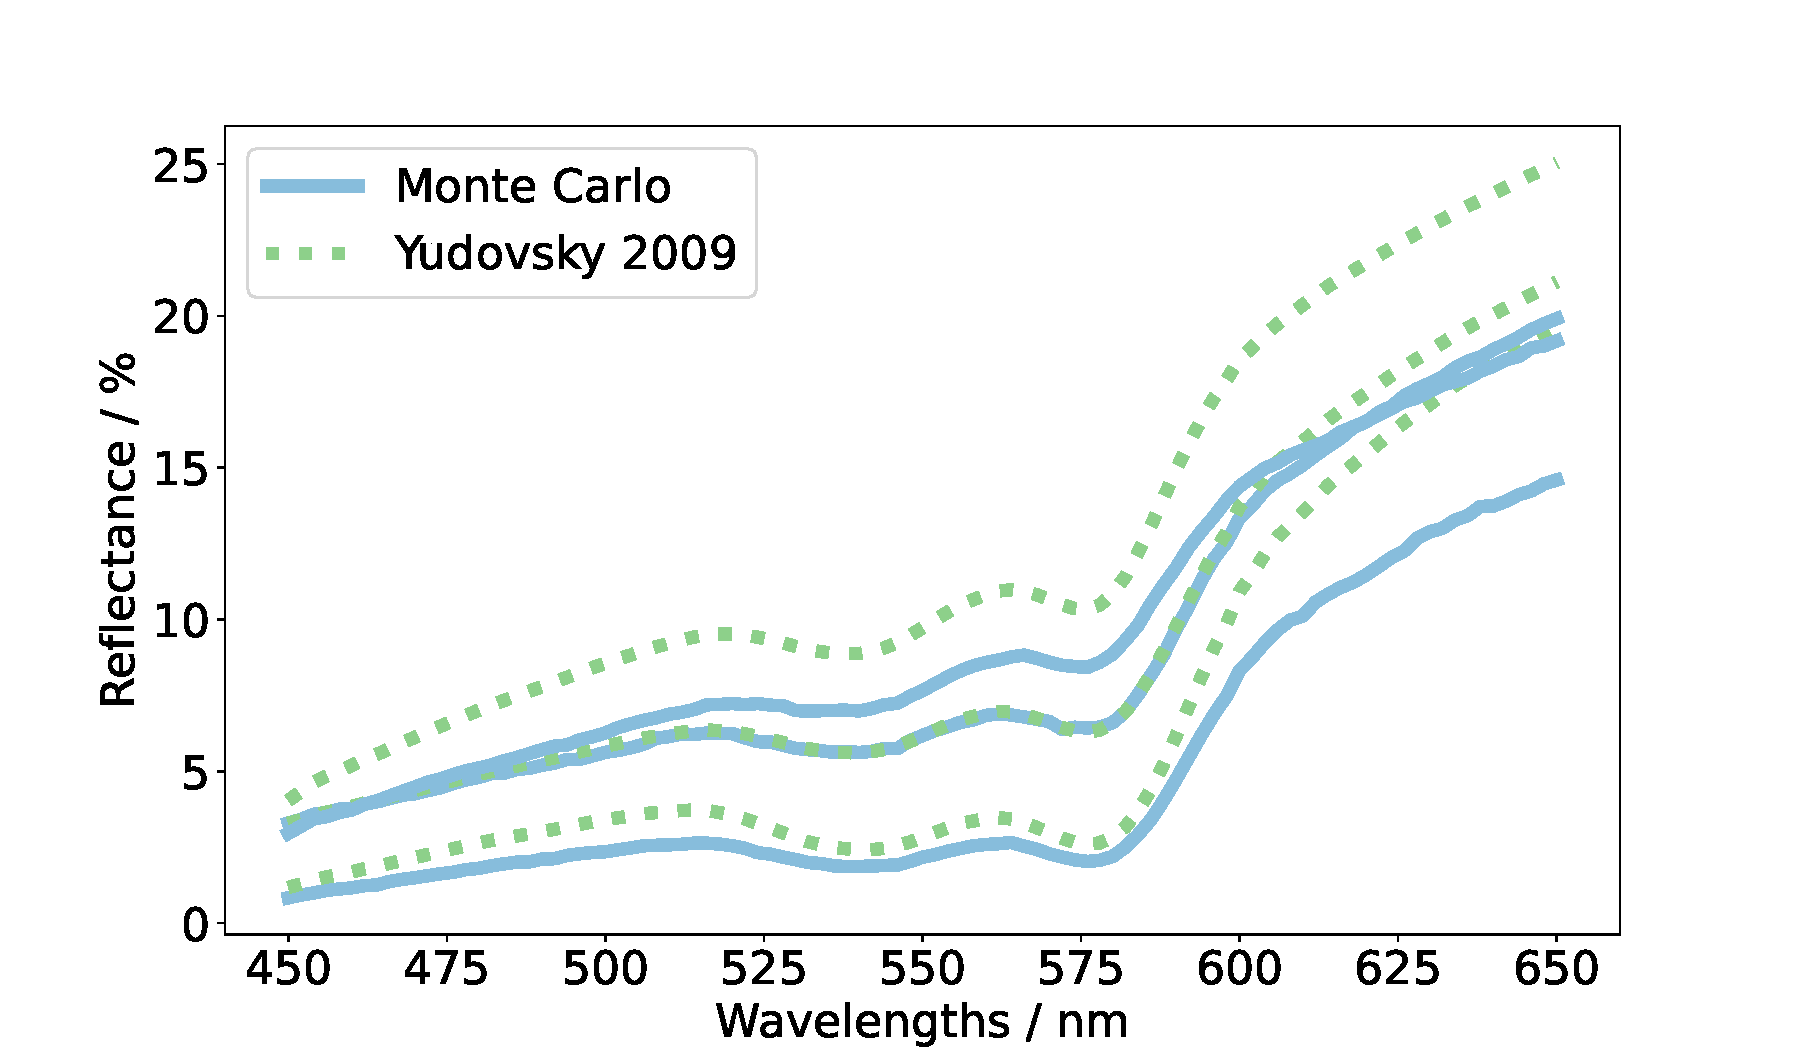
\includegraphics[width=\textwidth]{Compare_forwards_2_layer.pdf}
%         \caption{}
%         \label{fig:egtwolayerMCforwards}
%     \end{subfigure}
%     \begin{subfigure}{0.8\textwidth}
%         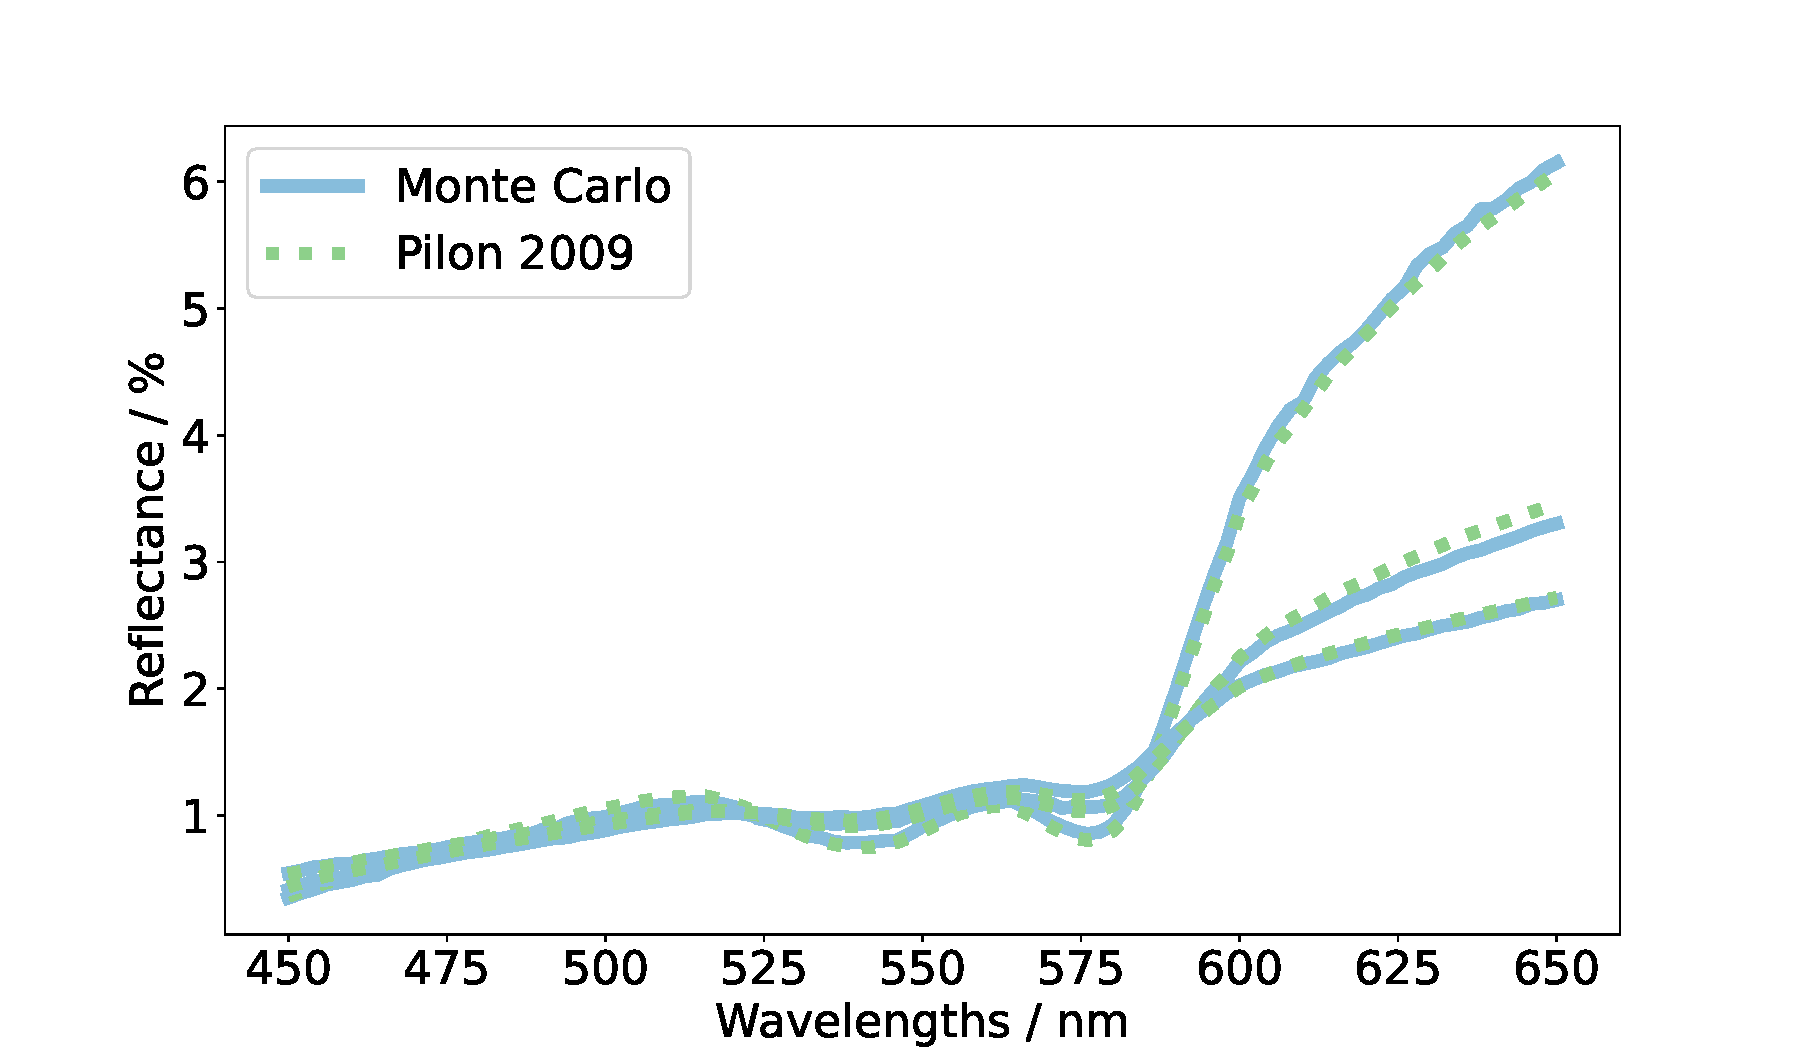
\includegraphics[width=\textwidth]{Compare_forwards_2_layer_norm.pdf}
%         \caption{}
%         \label{fig:egtwolayerMCforwardsnorm}
%     \end{subfigure}
%     \caption{Demonstration of the variability of quality of fit between the Yudovsky 2009 two layer model and Monte Carlo simulated diffuse spectra when using the same ground truth parameters for quantitative (left) or relative (right) data.}
%     \label{fig:MC2layerforwards}
% \end{figure}

% \begin{figure}[htbp]
%     \centering
%     \begin{subfigure}{0.8\textwidth}
%         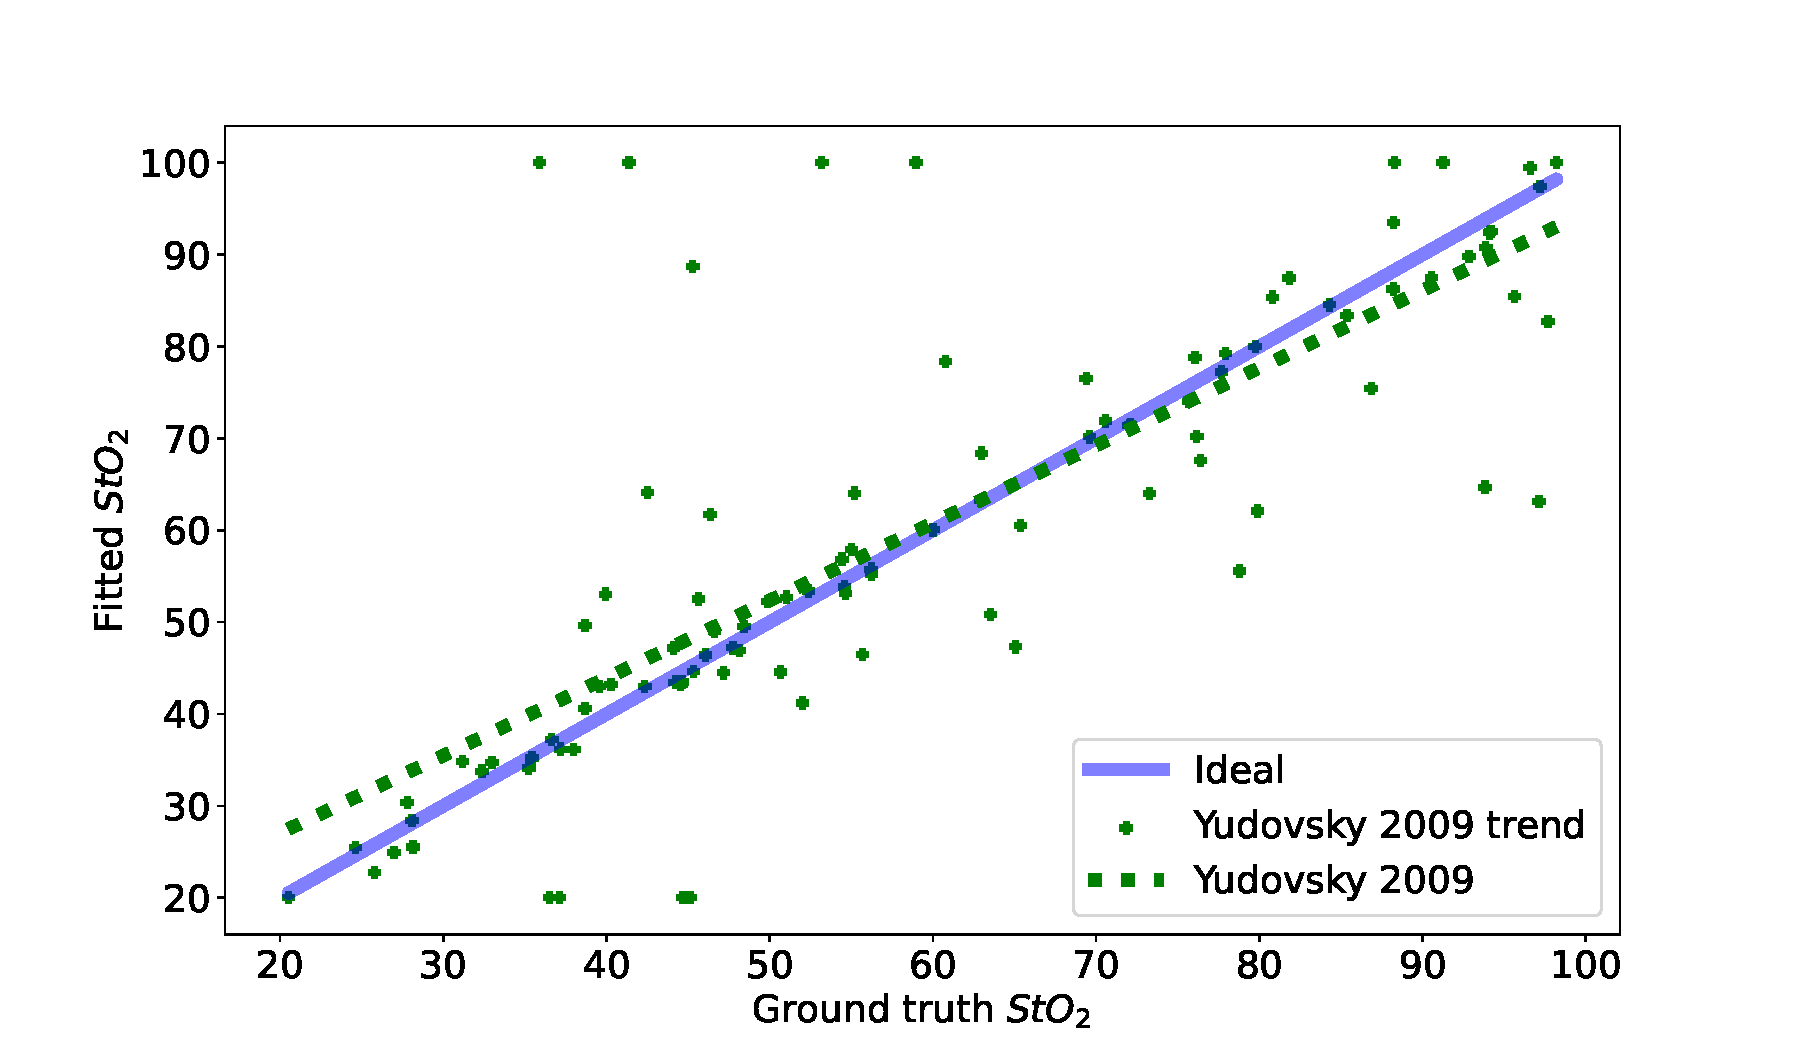
\includegraphics[width=\textwidth]{StO2_twolayer_MC.pdf}
%         \caption{}
%         \label{fig:egparamsStO2MC}
%     \end{subfigure}
%     \begin{subfigure}{0.8\textwidth}
%         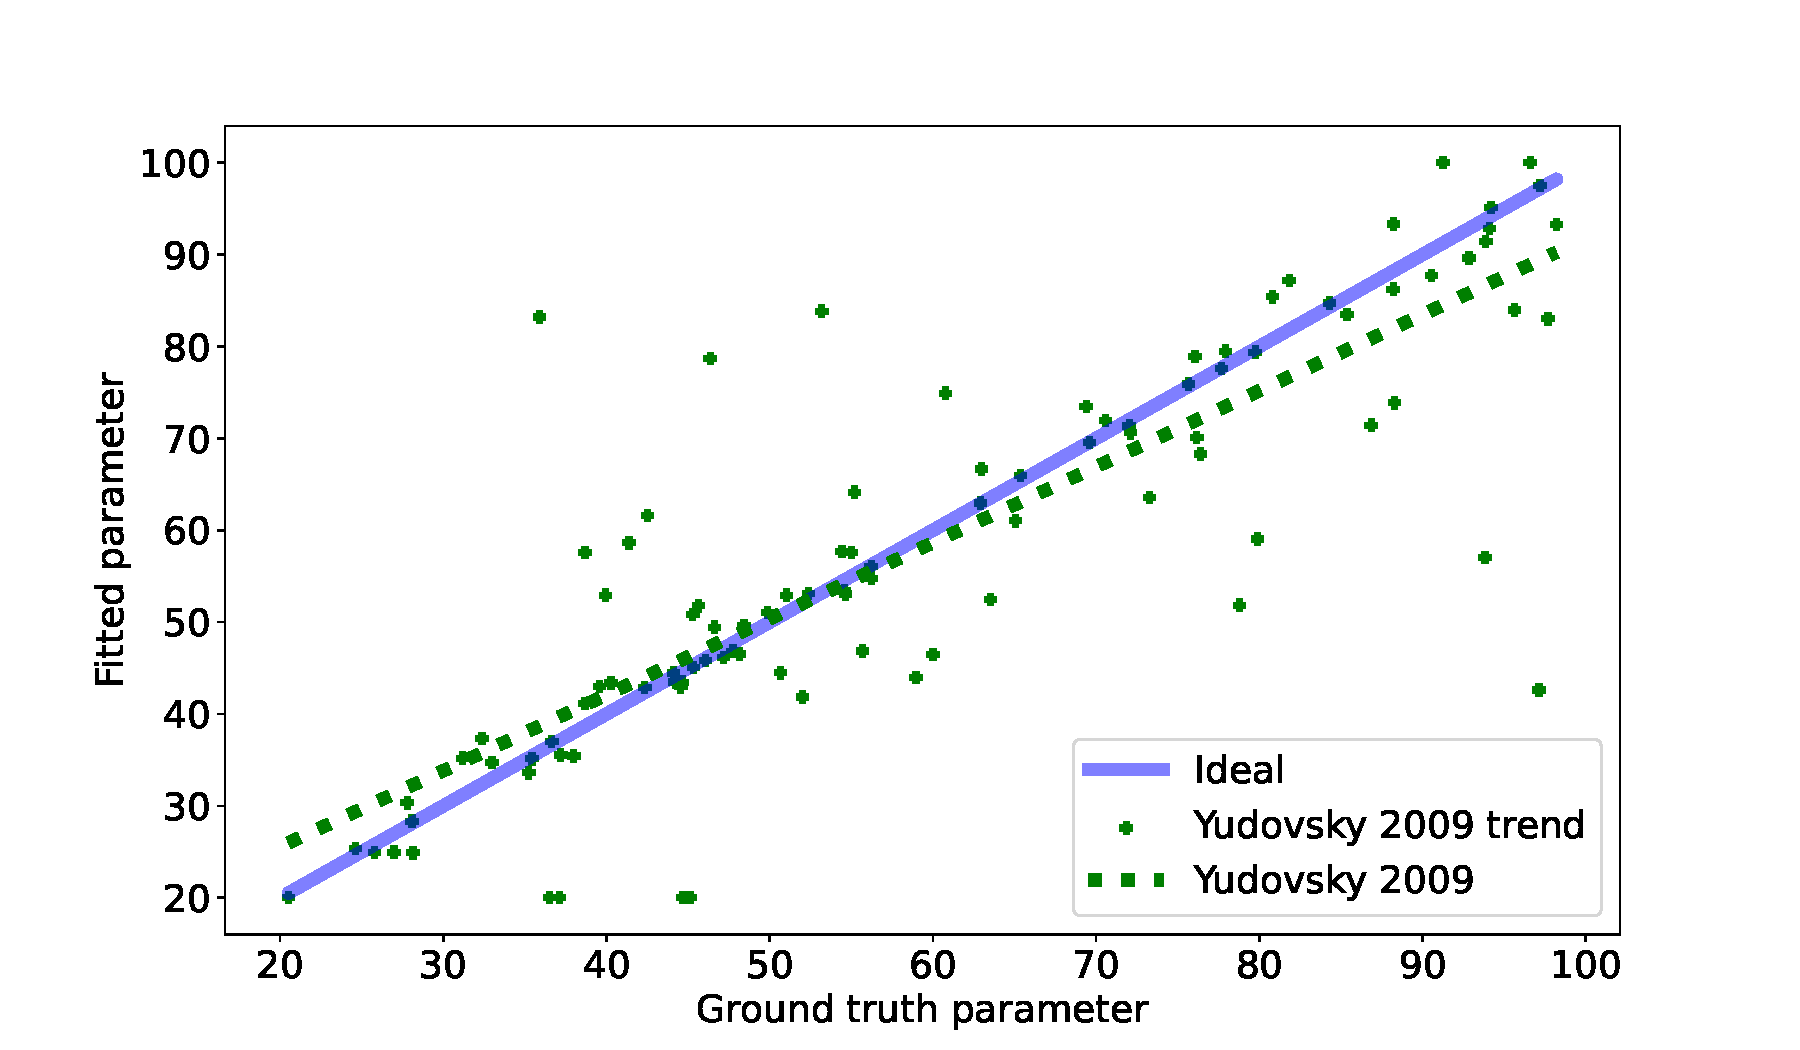
\includegraphics[width=\textwidth]{StO2_twolayer_MC_norm.pdf}
%         \caption{}
%         \label{fig:egparamsStO2MCnorm}
%     \end{subfigure}
%     \caption{Example $StO_2$ recovery from fitting Yudovsky 2009 two layer model to Monte Carlo simulated diffuse reflectance and the associated linear regression line between the extracted and ground truth parameters for quantitative (left) or relative (right) data.}
%     \label{fig:MC2layerinverse}
% \end{figure}

% \begin{figure}[htbp]
%     \centering
%     \begin{subfigure}{0.8\textwidth}
%         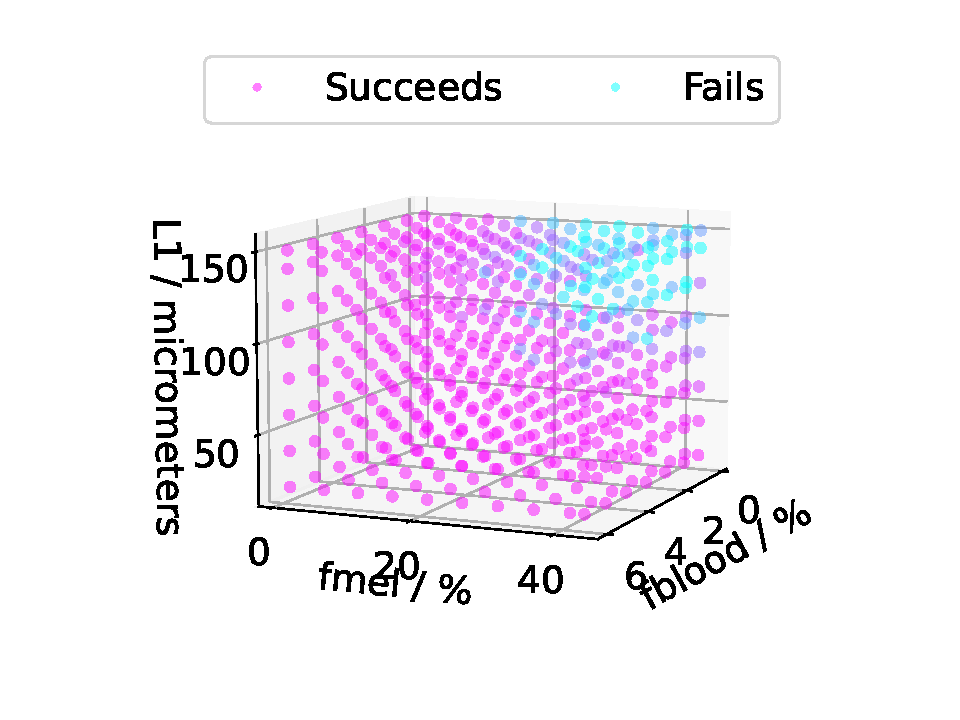
\includegraphics[width=\textwidth]{2layer_parameter_exploration.pdf}
%         \caption{}
%         \label{fig:egparamsfailureMC}
%     \end{subfigure}
%     \begin{subfigure}{0.8\textwidth}
%         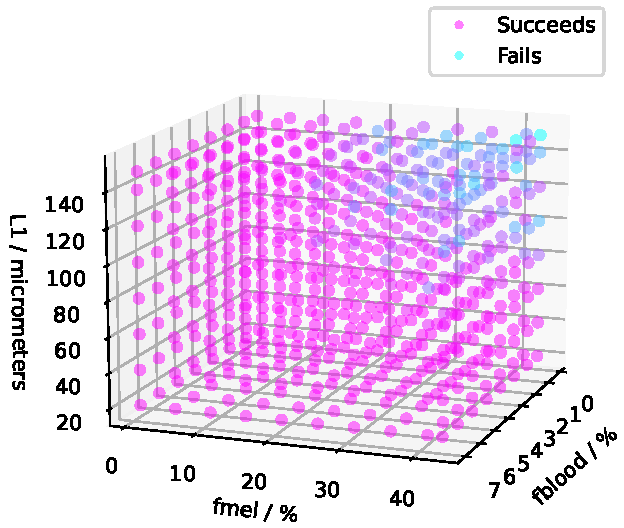
\includegraphics[width=\textwidth]{2layer_parameter_exploration_norm.pdf}
%         \caption{}
%         \label{fig:egparamsfailureMCnorm}
%     \end{subfigure}
%     \caption{A depiction of the impact of 3 key physiological parameters on success of $StO_2$ extraction by Yudovsky 2009 two layer model for quantitative (left) or relative (right) data.}
%     \label{fig:MC2layerfailure}
% \end{figure}

\begin{figure}[htbp]
    \centering
    \begin{subfigure}{0.49\textwidth}
        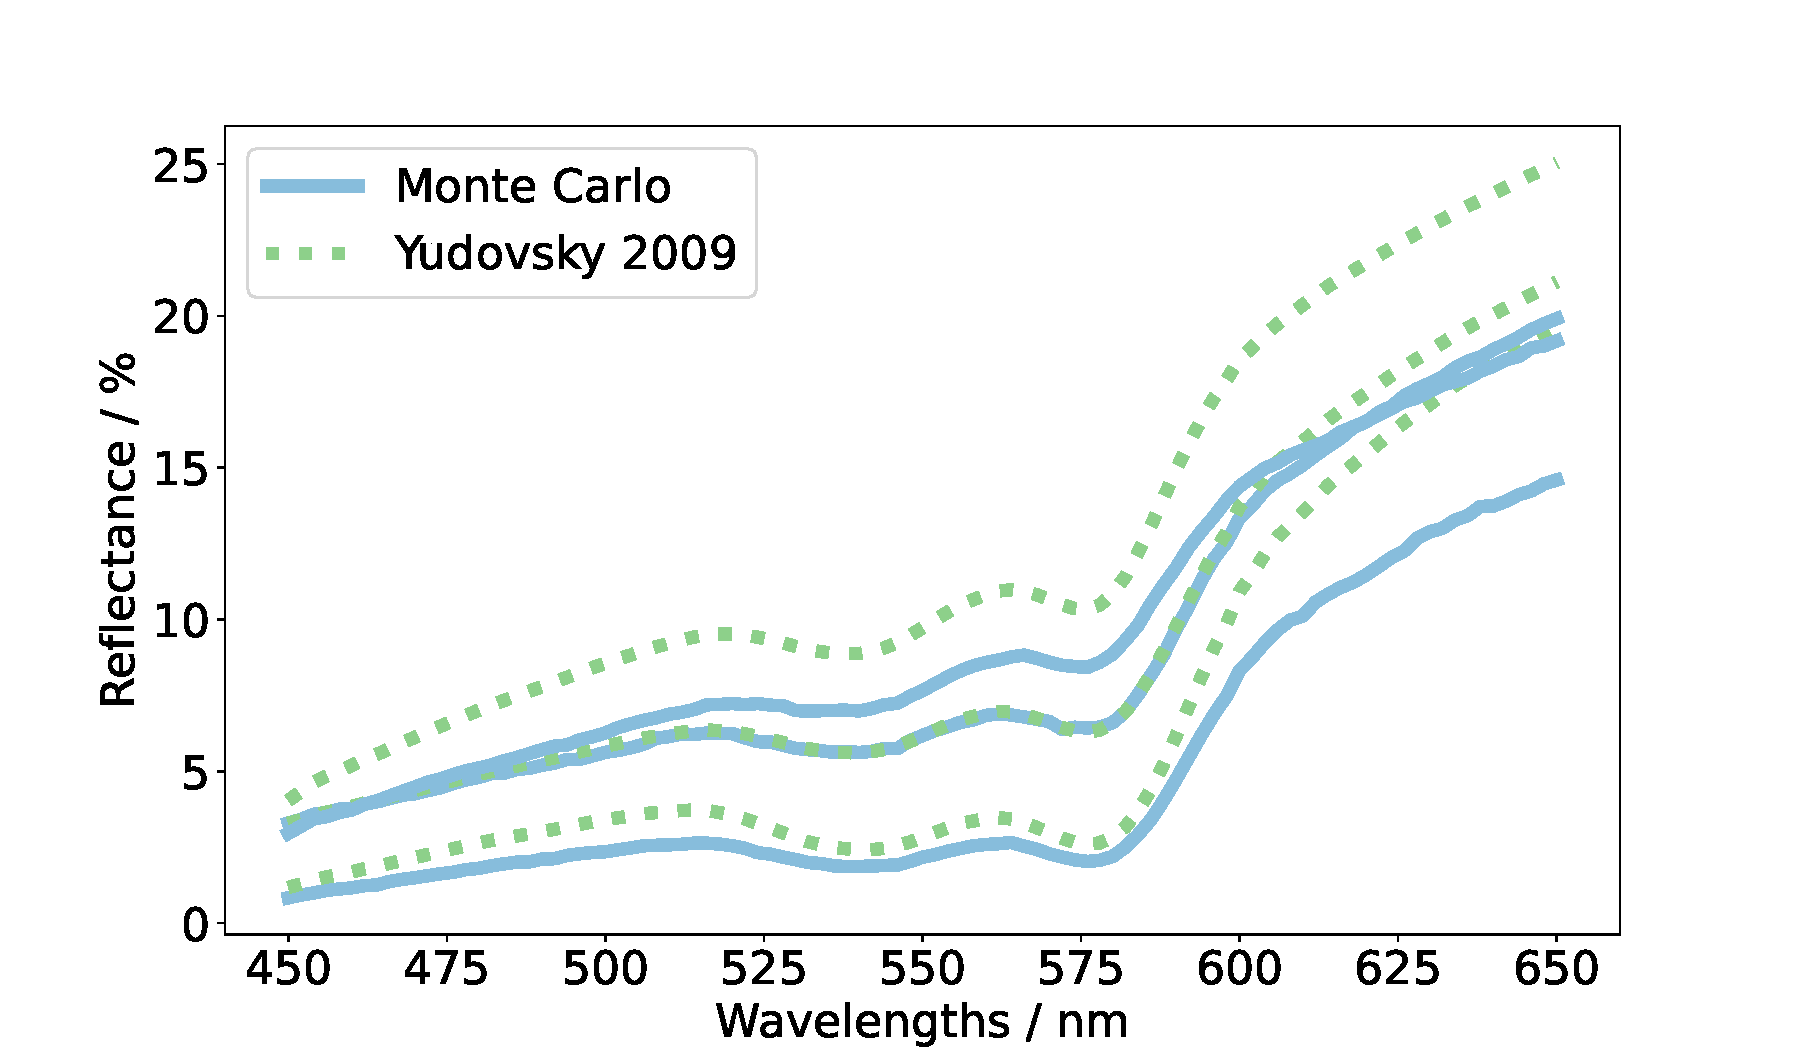
\includegraphics[width=\textwidth]{Compare_forwards_2_layer.pdf}
        \caption{}
        \label{fig:egtwolayerMCforwards}
    \end{subfigure}
    \begin{subfigure}{0.49\textwidth}
        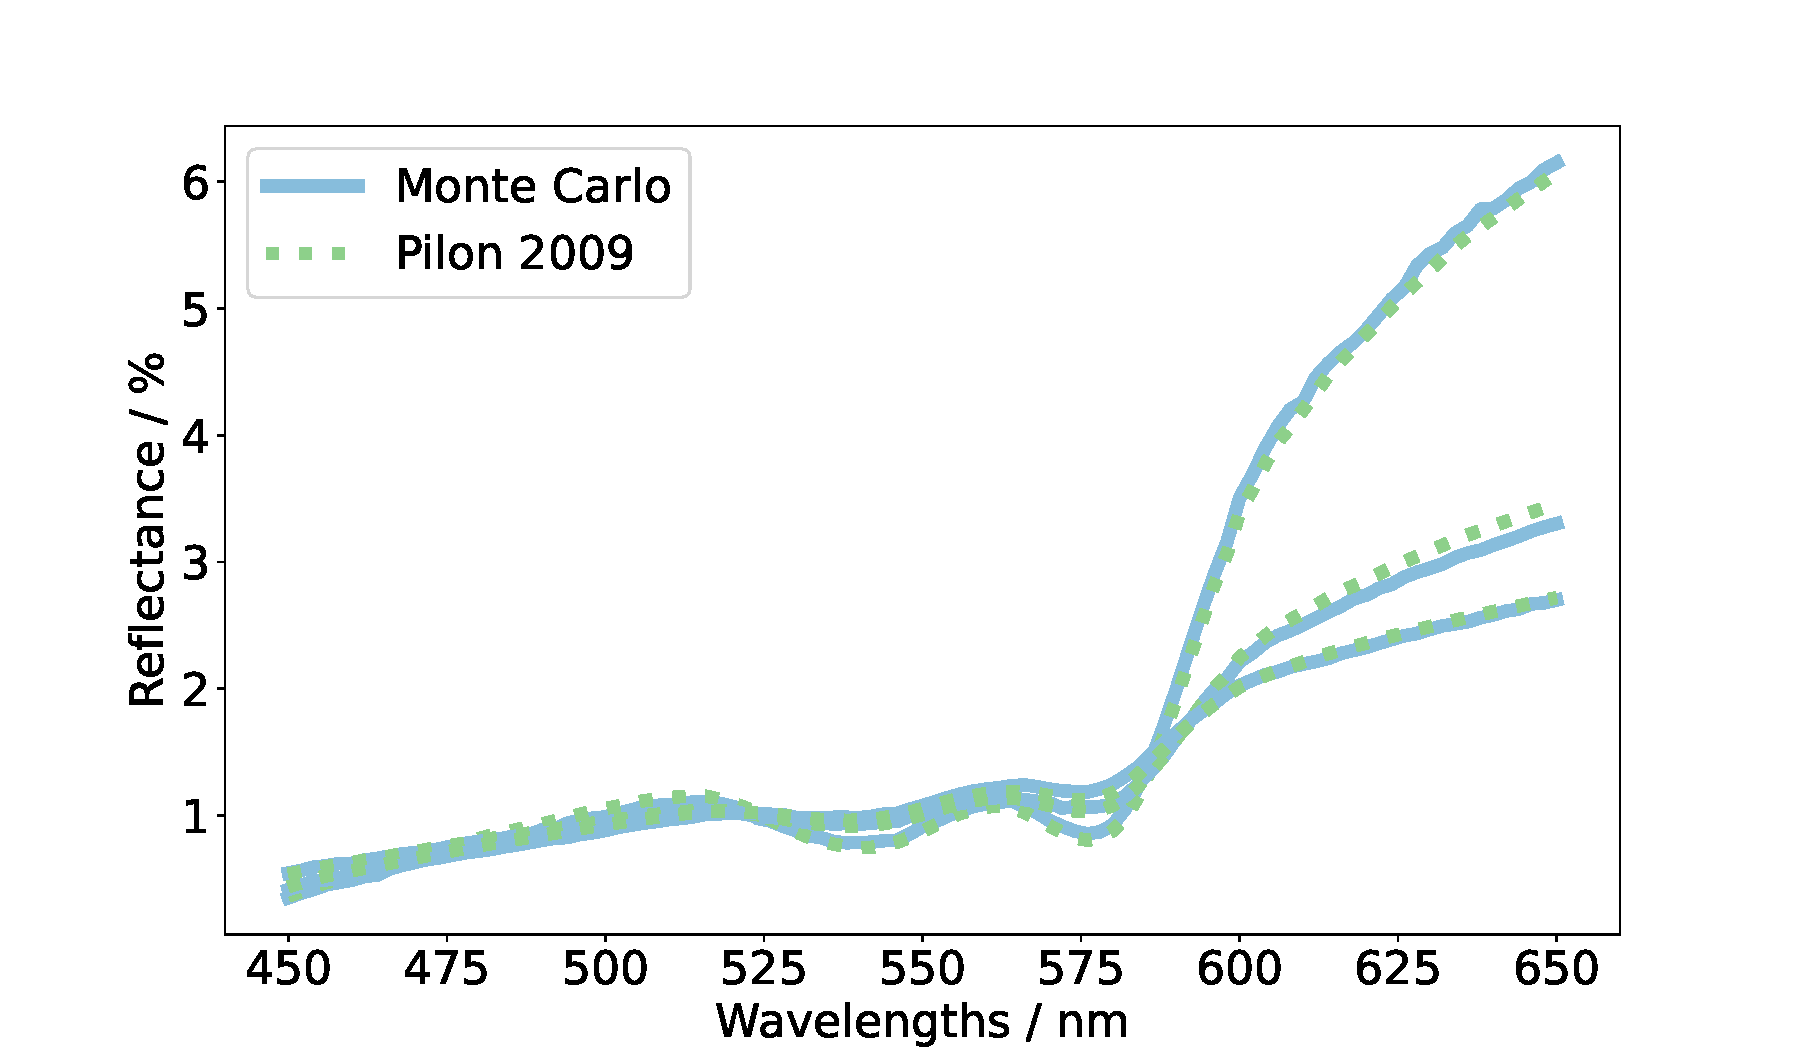
\includegraphics[width=\textwidth]{Compare_forwards_2_layer_norm.pdf}
        \caption{}
        \label{fig:egtwolayerMCforwardsnorm}
    \end{subfigure}
    \begin{subfigure}{0.49\textwidth}
        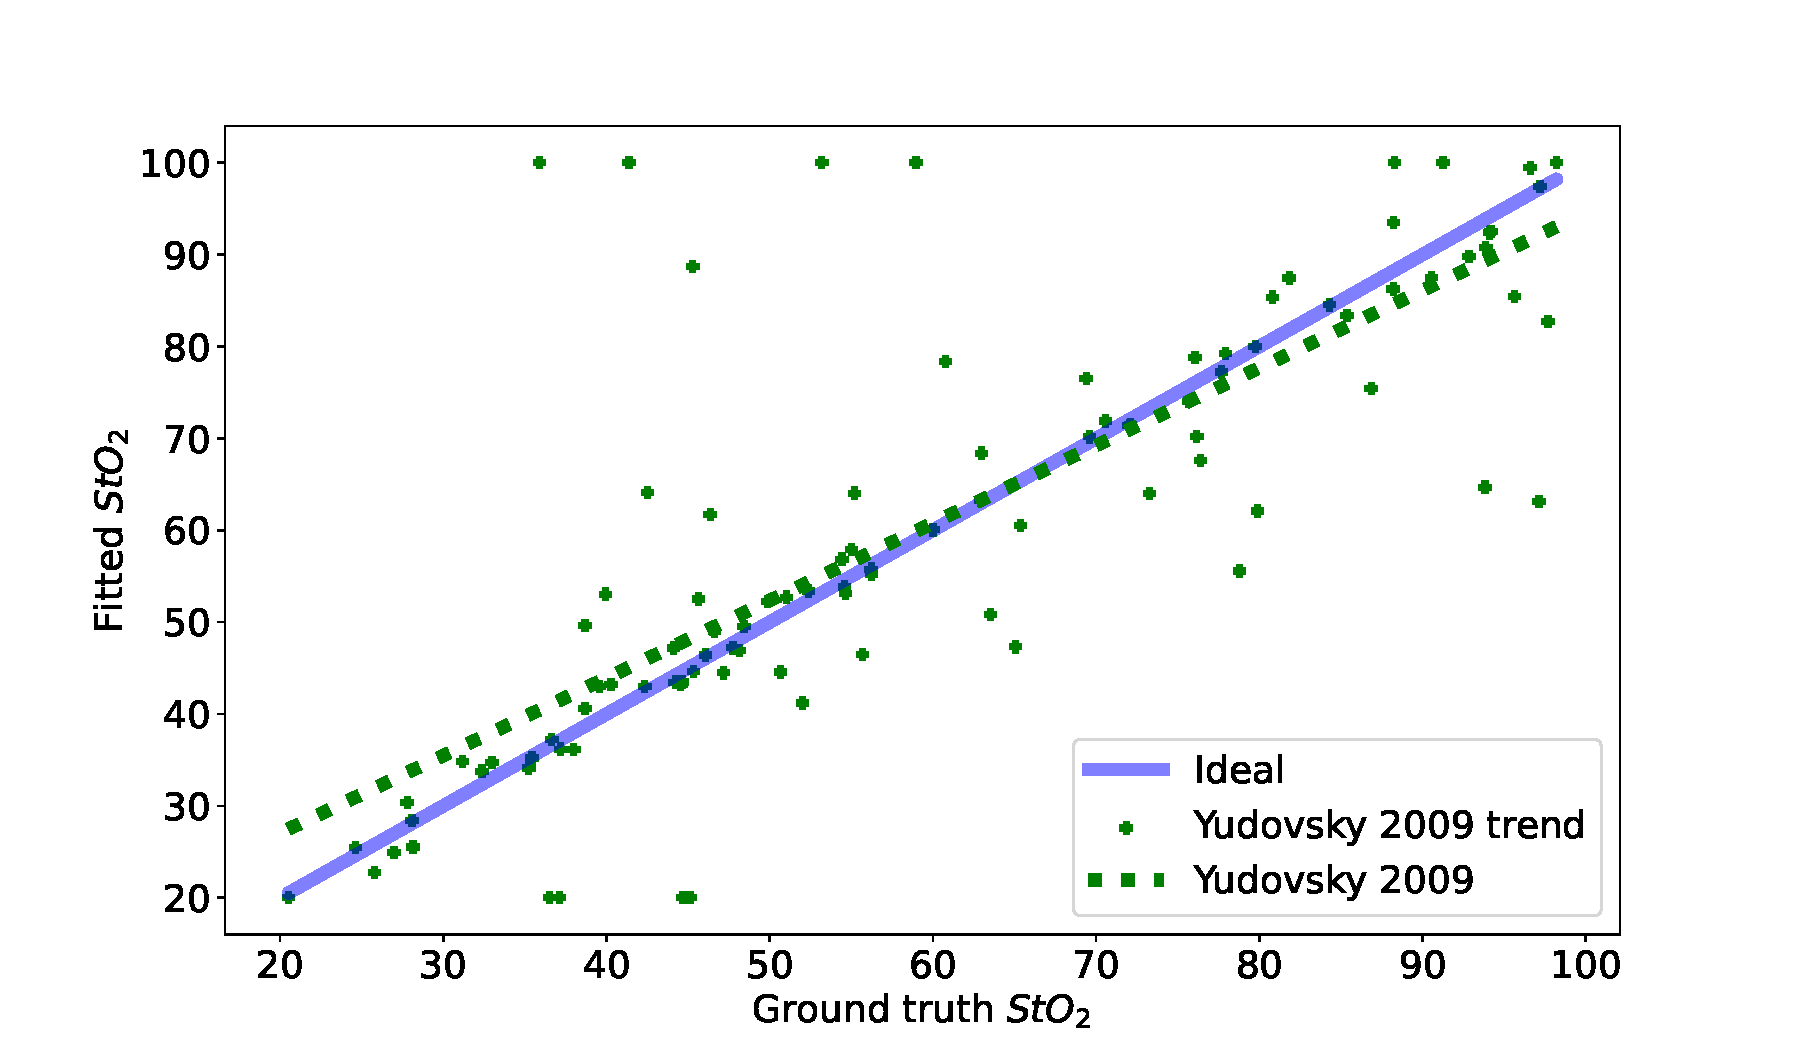
\includegraphics[width=\textwidth]{StO2_twolayer_MC.pdf}
        \caption{}
        \label{fig:egparamsStO2MC}
    \end{subfigure}
    \begin{subfigure}{0.49\textwidth}
        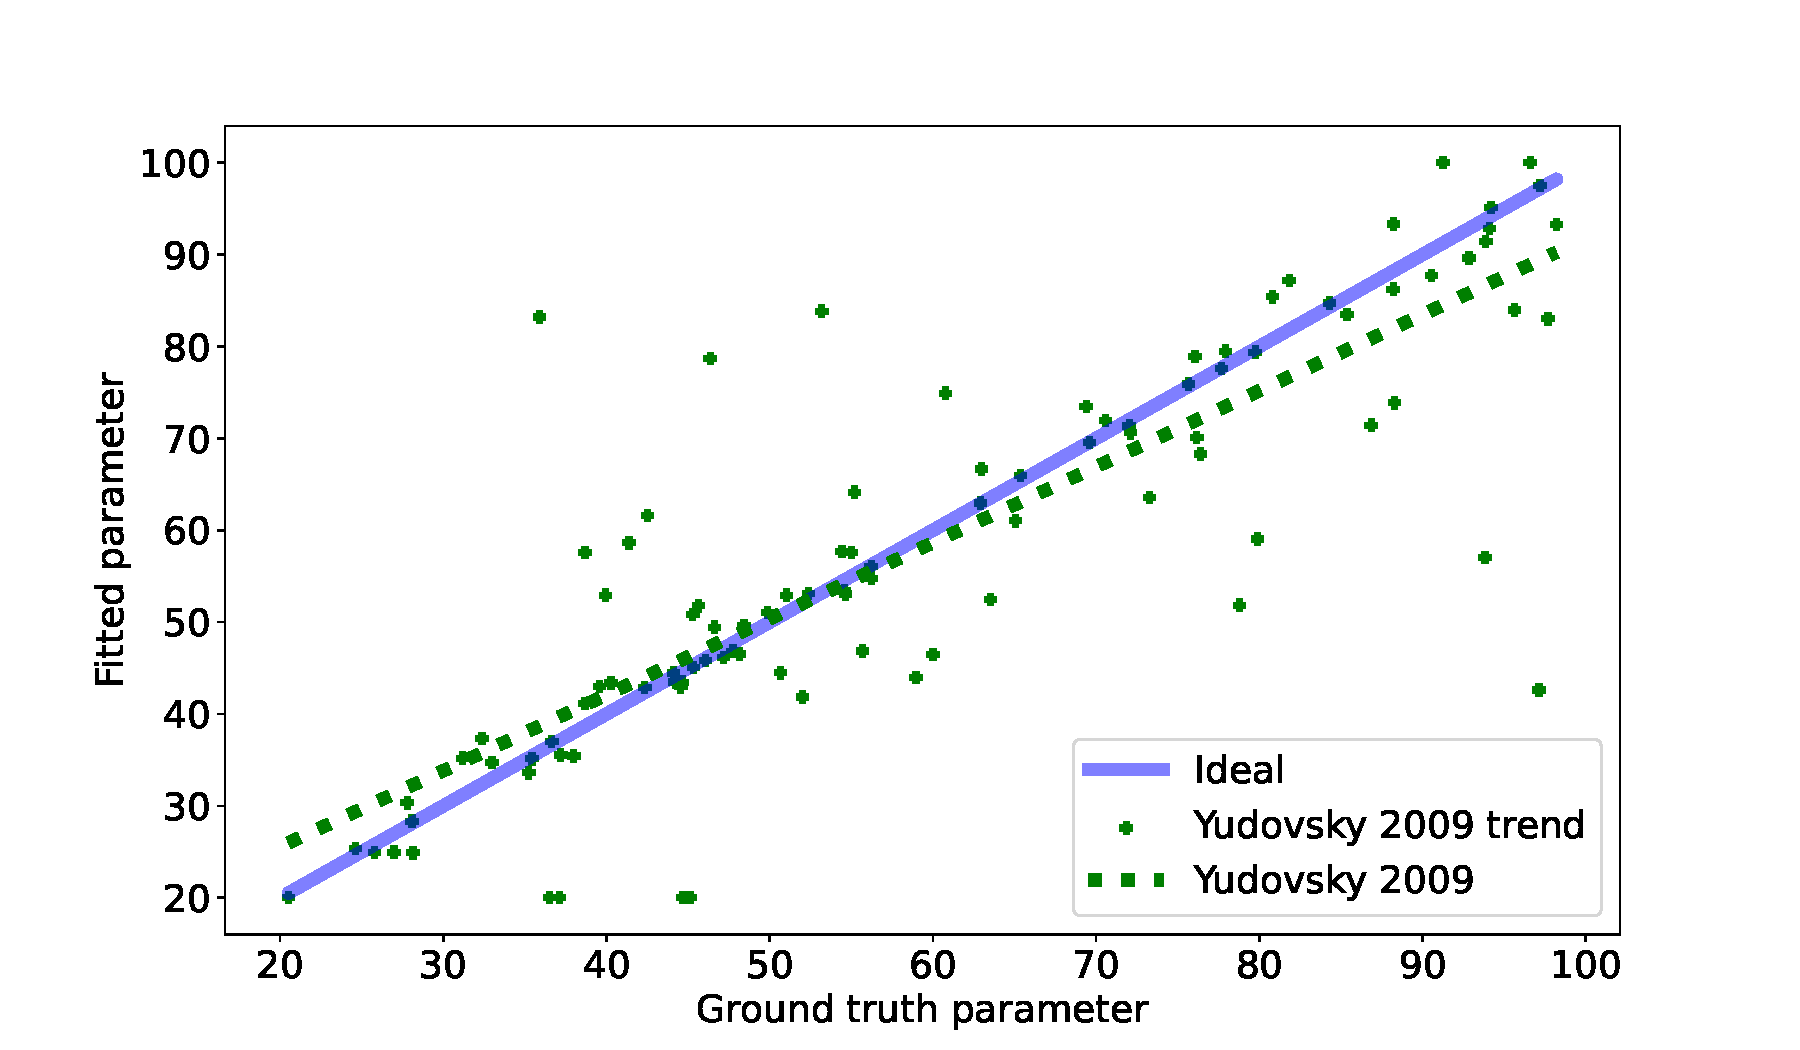
\includegraphics[width=\textwidth]{StO2_twolayer_MC_norm.pdf}
        \caption{}
        \label{fig:egparamsStO2MCnorm}
    \end{subfigure}
    \begin{subfigure}{0.49\textwidth}
        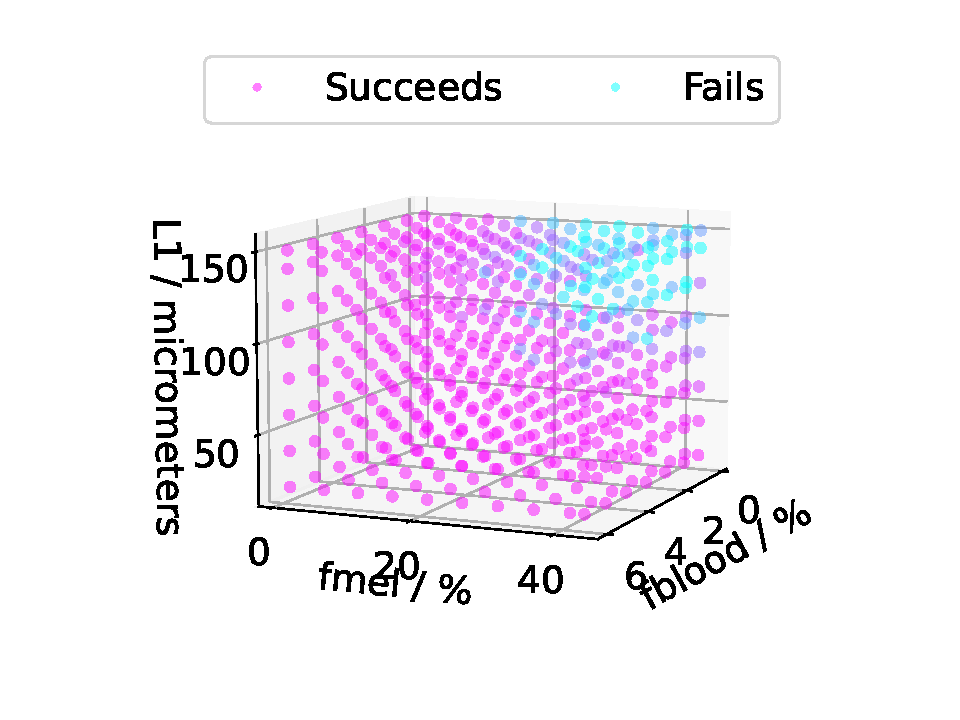
\includegraphics[width=\textwidth]{2layer_parameter_exploration.pdf}
        \caption{}
        \label{fig:egparamsfailureMC}
    \end{subfigure}
    \begin{subfigure}{0.49\textwidth}
        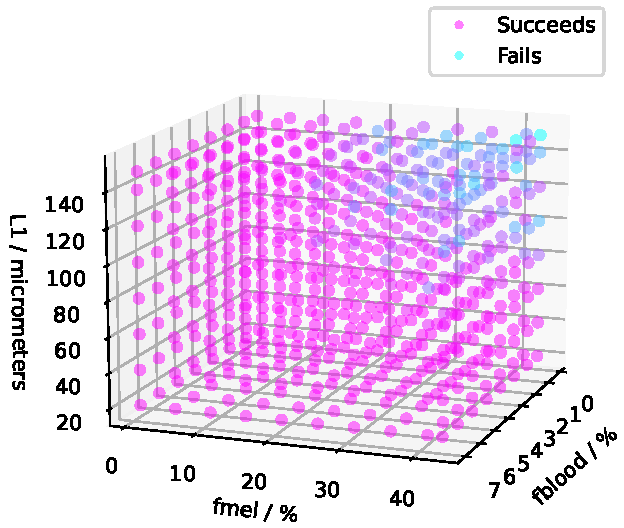
\includegraphics[width=\textwidth]{2layer_parameter_exploration_norm.pdf}
        \caption{}
        \label{fig:egparamsfailureMCnorm}
    \end{subfigure}
    \caption{Top: Demonstration of the variability of quality of fit between the Yudovsky 2009 two layer model and Monte Carlo simulated diffuse spectra when using the same ground truth parameters for quantitative (left) or relative (right) data. Middle: Example $StO_2$ recovery from fitting Yudovsky 2009 two layer model to Monte Carlo simulated diffuse reflectance and the associated linear regression line between the extracted and ground truth parameters for quantitative (left) or relative (right) data. Bottom: a depiction of the impact of 3 key physiological parameters on success of $StO_2$ extraction by Yudovsky 2009 two layer model for quantitative (left) or relative (right) data.}
    \label{fig:MC2layer}
\end{figure}

When fitting the model to the Monte Carlo dataset, the $a$, $b$, $StO_2$, $f_{blood}$, $f_{mel}$, and $L_1$ parameters are extracted and compared to the ground truth Monte Carlo inputs using a linear regression. The regression gradient ($m$) and offset ($c$) between these retrieved values and the ground truth counterparts, alongside the Pearson $r$ values (bold if $p$ is significant), and the mean ($\pm$ standard deviation) absolute percentage errors are shown in Table \ref{tb:doubleparamtrends}. An example of the fitted parameters compared to the ground truth parameters is shown for $StO_2$ in Figure \ref{fig:egparamsStO2MC} for quantitative data and Figure \ref{fig:egparamsStO2MCnorm} for relative data. This shows parameter extraction to be significantly poorer than for the single-layer model and parameter extraction from quantitative data performing similarly that of relative data for $StO_2$ but better for all others. 
\begin{table}[h]
    \centering
    \caption{The regression gradient $m$, offset $c$, Pearson $r$ (bold if $p$<0.05), and the mean ($\pm$ standard deviation) absolute percentage errors ($APE$) for each variable when extracted by fitting Yudovsky 2009 two layer model to the quantitative (Q) or relative (R) Monte-Carlo diffuse reflectance dataset. All presented to 3s.f.}
    \begin{tabular}{|c|c|cccc|}
        \hline
        Parameter & Quantitative (Q) & $m$ & $c$ & $r$ & mean ($\pm$  \\
        & or Relative (R) & (ideal =1) & (ideal = 0) & (ideal = 1) & standard deviation) \\
        & & & & & $APE$ (\%) \\
        \hline
        \multirow{2}{*}{$StO_2$} & Q & 0.844 & 10.2 & \textbf{0.788} & 15.3($\pm$ 27.5) \\
        & R & 0.827 & 8.99 & \textbf{0.836} & 13.1($\pm$ 19.7) \\
        \hline
        \multirow{2}{*}{$f_{blood}$} & Q & 0.948 & 0.270 & \textbf{0.852} & 24.0($\pm$ 23.9) \\
        & R & 0.784 & 0.216 & \textbf{0.672} & 32.4($\pm$ 27.8) \\
        \hline
        \multirow{2}{*}{$f_{mel}$} & Q & 0.842 & 1.38 & \textbf{0.843} & 27.0($\pm$ 25.7) \\
        & R & 0.502 & 5.14 & \textbf{0.506} & 38.1($\pm$ 24.6) \\
        \hline
        \multirow{2}{*}{$L_1$} & Q & 0.825 & 31.4 & \textbf{0.794} & 38.6($\pm$ 41.9) \\
         & R & 0.798 & 37.7 & \textbf{0.775} & 41.6($\pm$ 39.9) \\
        \hline
        \multirow{2}{*}{$a$} & Q & 0.752 & 11.2 & \textbf{0.617} & 20.0($\pm$ 15.5) \\
        & R & 0.445 & 24.0 & \textbf{0.333} & 28.0($\pm$ 24.6) \\
        \hline
        \multirow{2}{*}{$b$} & Q & 0.826 & 0.286 & \textbf{0.739} & 16.4($\pm$ 18.5) \\
        & R & 0.710 & 0.530 & \textbf{0.509} & 29.6($\pm$ 31.4) \\
        \hline
    \end{tabular}
    \label{tb:doubleparamtrends}
\end{table}
Graphs shown in Figure \ref{fig:egparamsfailureMC} (for quantitative) and Figure \ref{fig:egparamsfailureMCnorm} (for relative) demonstrate the impact of each parameter on model success for $StO_2$ parameter extraction when a singular ground truth scattering is fixed. This shows that the effect of $StO_2$ on the diffuse reflectance spectrum is masked by the melanin effect in areas of low $f_{blood}$, or high $L_1$ or $f_{mel}$ leading to poor $StO_2$ extraction in these areas. 
\FloatBarrier

\subsection{NIST}\label{sec:resultsNIST}
The inverse Yudovsky two layer model is compared to a NIST skin total reflectance dataset. The weighting function in Figure \ref{fig:weighting} is used to ensure good fitting and a refractive index of 1.44 is assumed for tissue in the visible range \cite{Yudovsky2009}. 

There are no ground truth parameters for these measured spectra, however the $a$, $b$, $StO_2$, $f_{blood}$, $f_{mel}$, and $L_1$ parameters are extracted and the mean($\pm$ standard deviation) is compared to expected values for healthy individuals \cite{Jacques2013, VanManen2021, Nishidate2011, Lintzeri2022} in Table \ref{tb:NISTparams} for quantitative (Q) and relative (R) data. This demonstrates that overall fitting to relative data performs better than quantitative data, however neither is able to recover $StO_2$ well. 
% \begin{figure}[h]
%     \centering
%     \begin{subfigure}{0.8\textwidth}
%         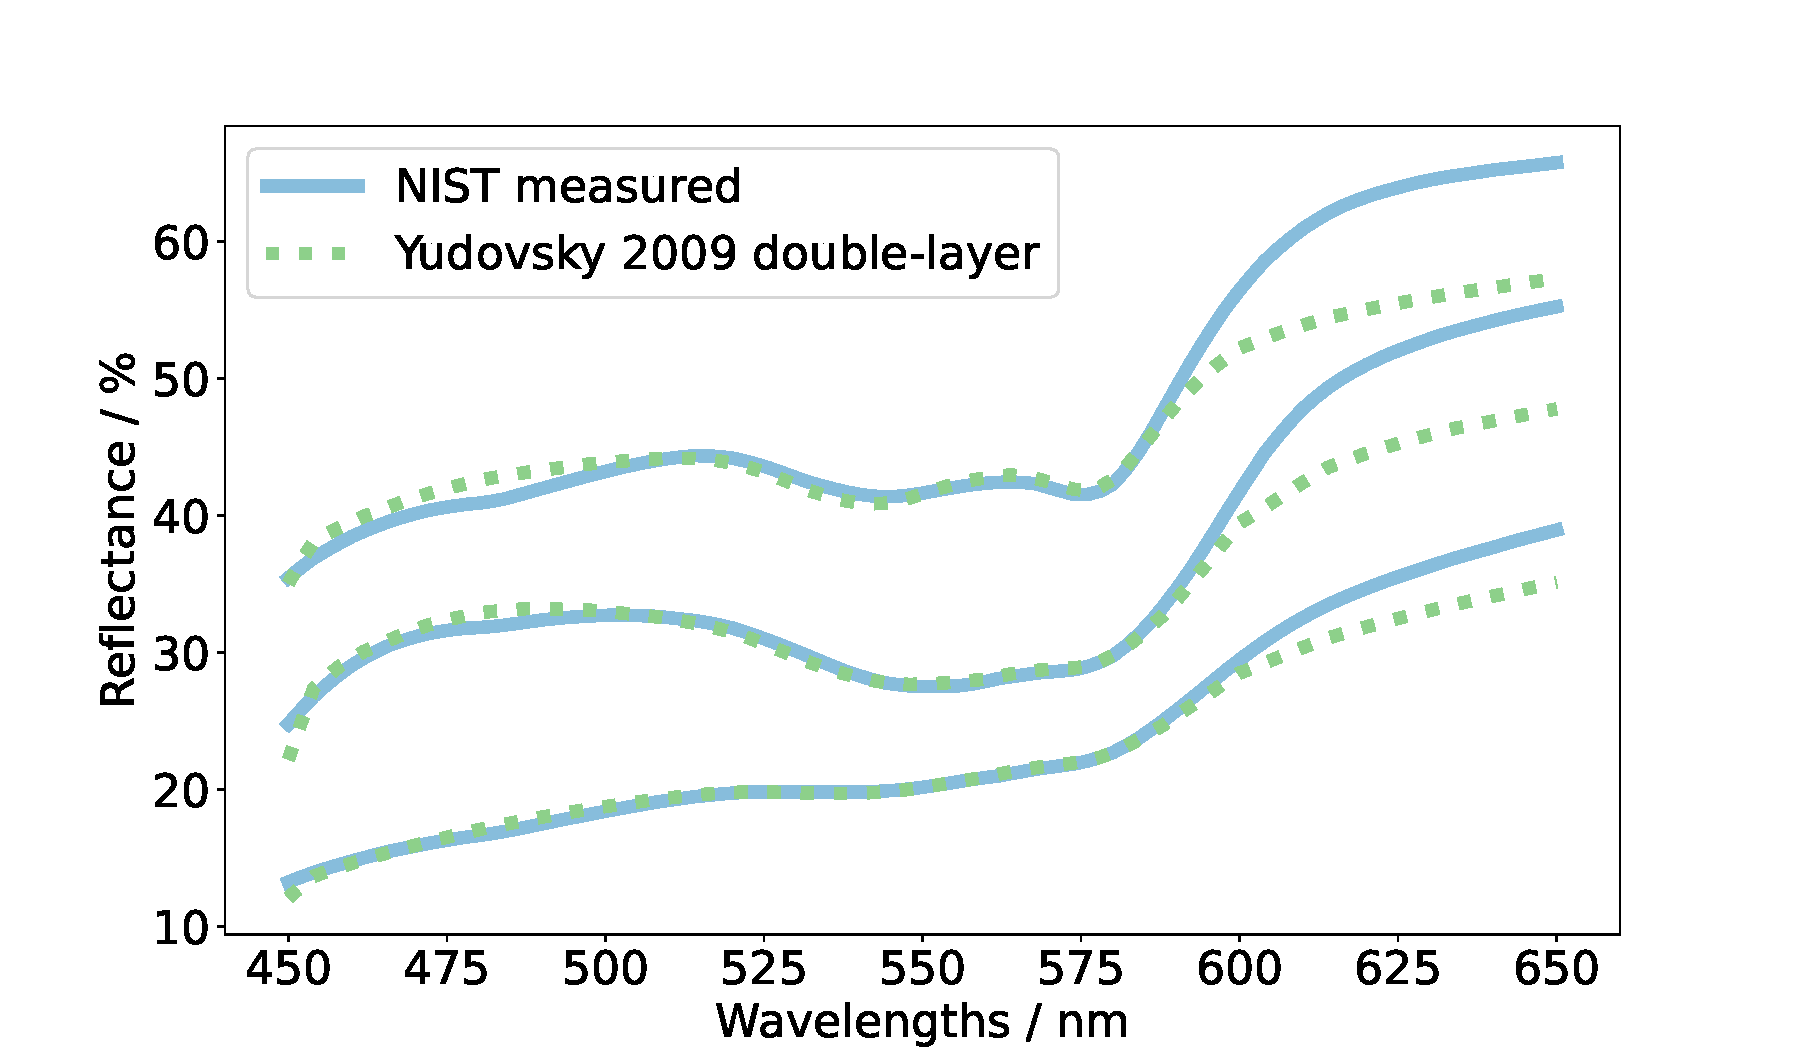
\includegraphics[width=\textwidth]{NIST_Eg.pdf}
%         \caption{}
%         \label{fig:egspectraNIST}
%     \end{subfigure}
%     \begin{subfigure}{0.8\textwidth}
%         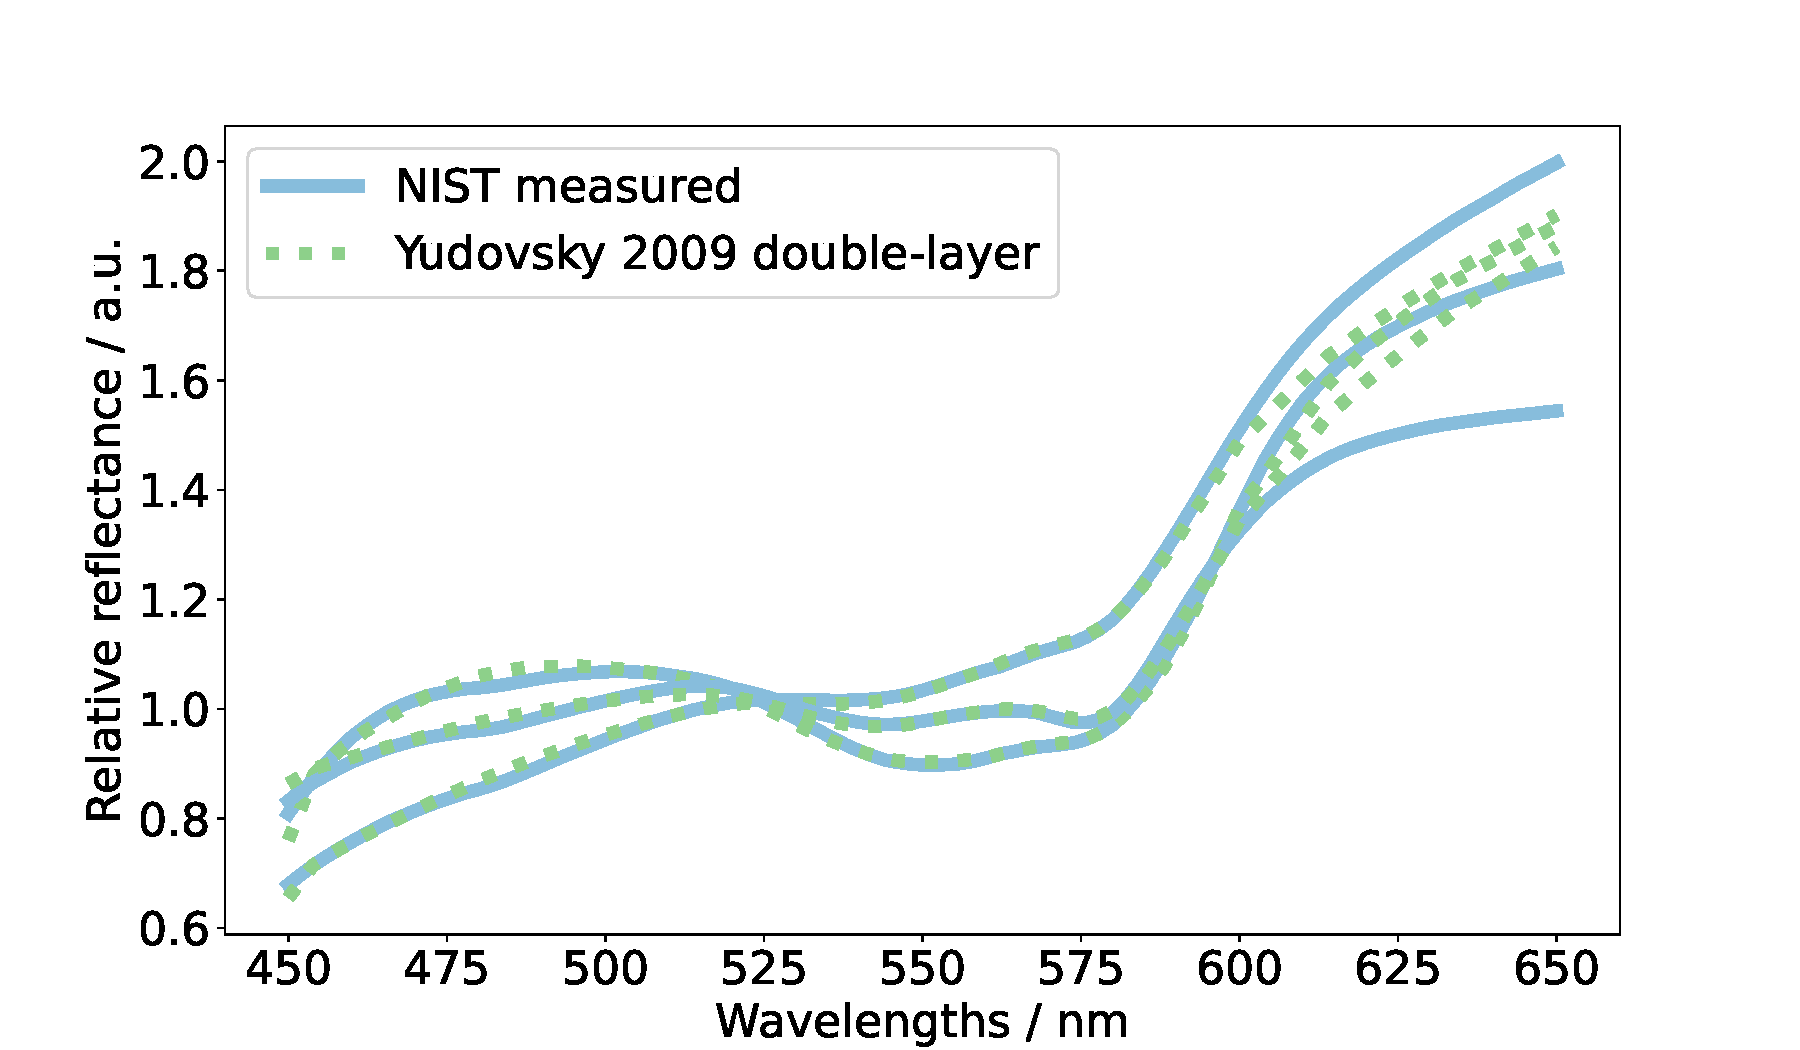
\includegraphics[width=\textwidth]{NIST_Eg_norm.pdf}
%         \caption{}
%         \label{fig:egspectraNISTnorm}
%     \end{subfigure}
%     % \begin{subfigure}{0.49\textwidth}
%     %     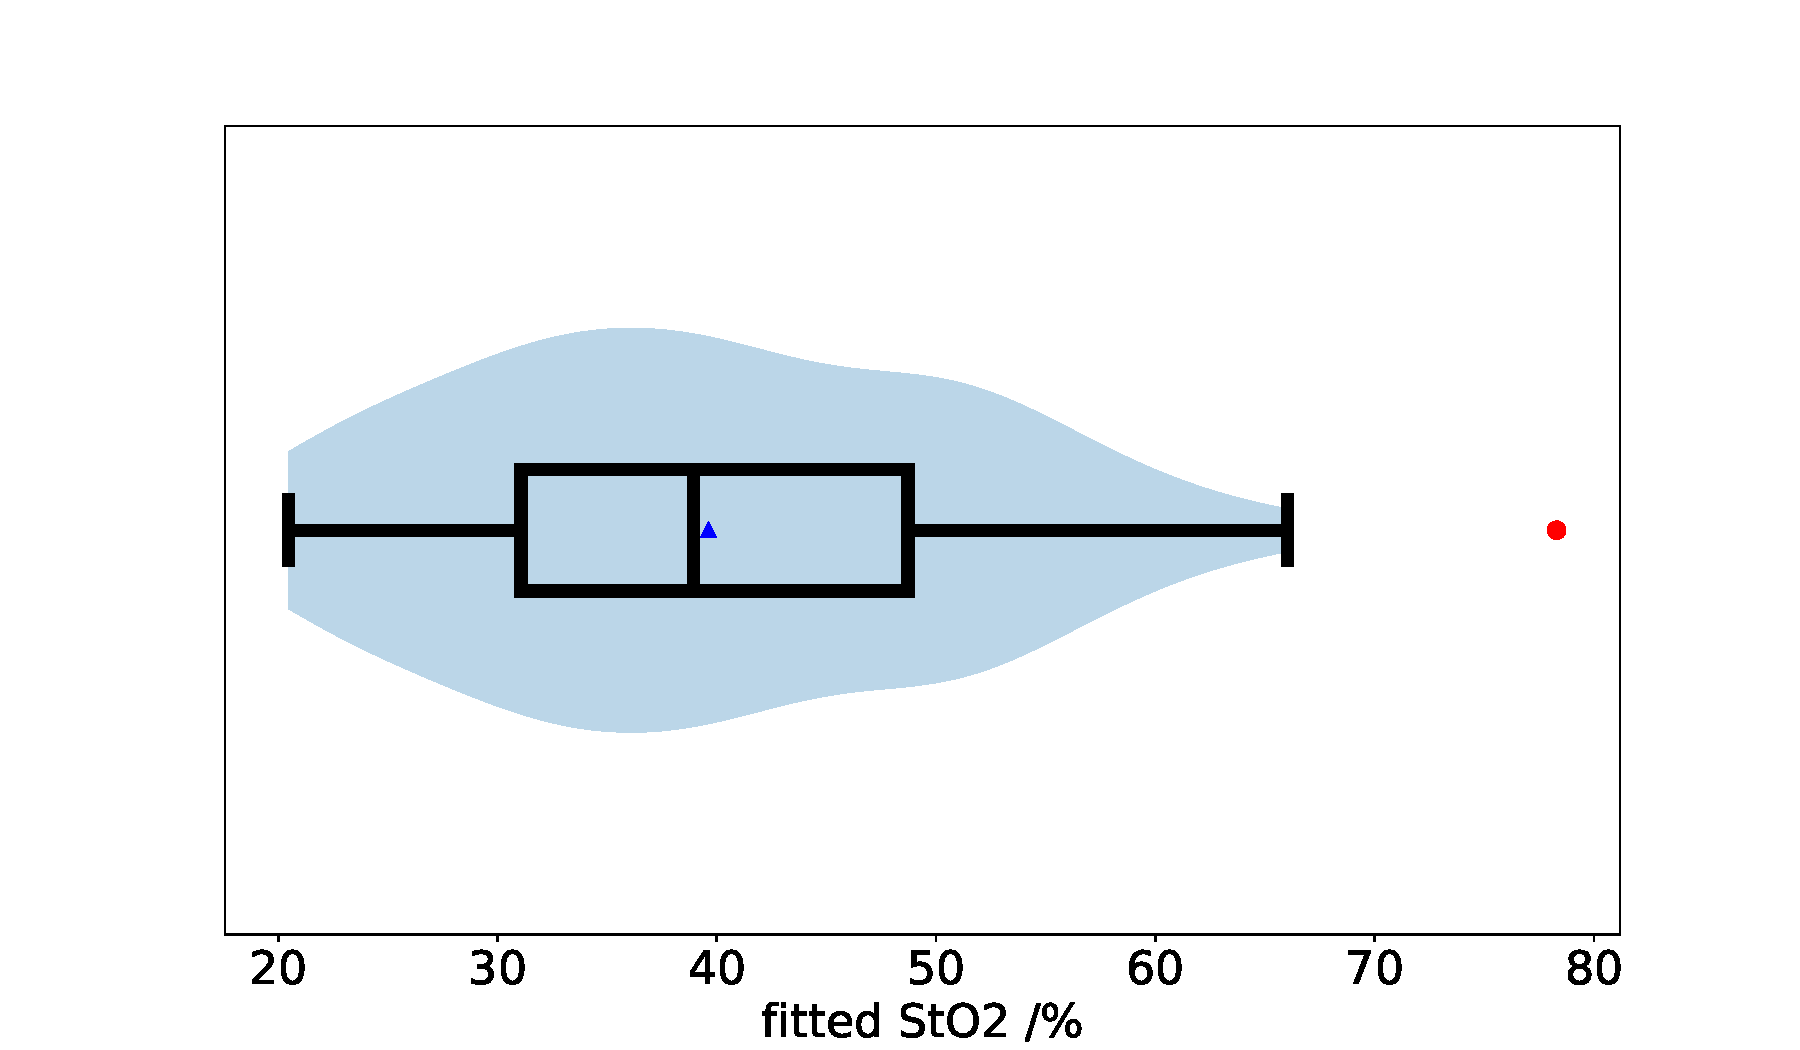
\includegraphics[width=\textwidth]{StO2_boxplot.pdf}
%     %     \caption{}
%     %     \label{fig:egparamStO2NIST}
%     % \end{subfigure}
%     % \begin{subfigure}{0.49\textwidth}
%     %     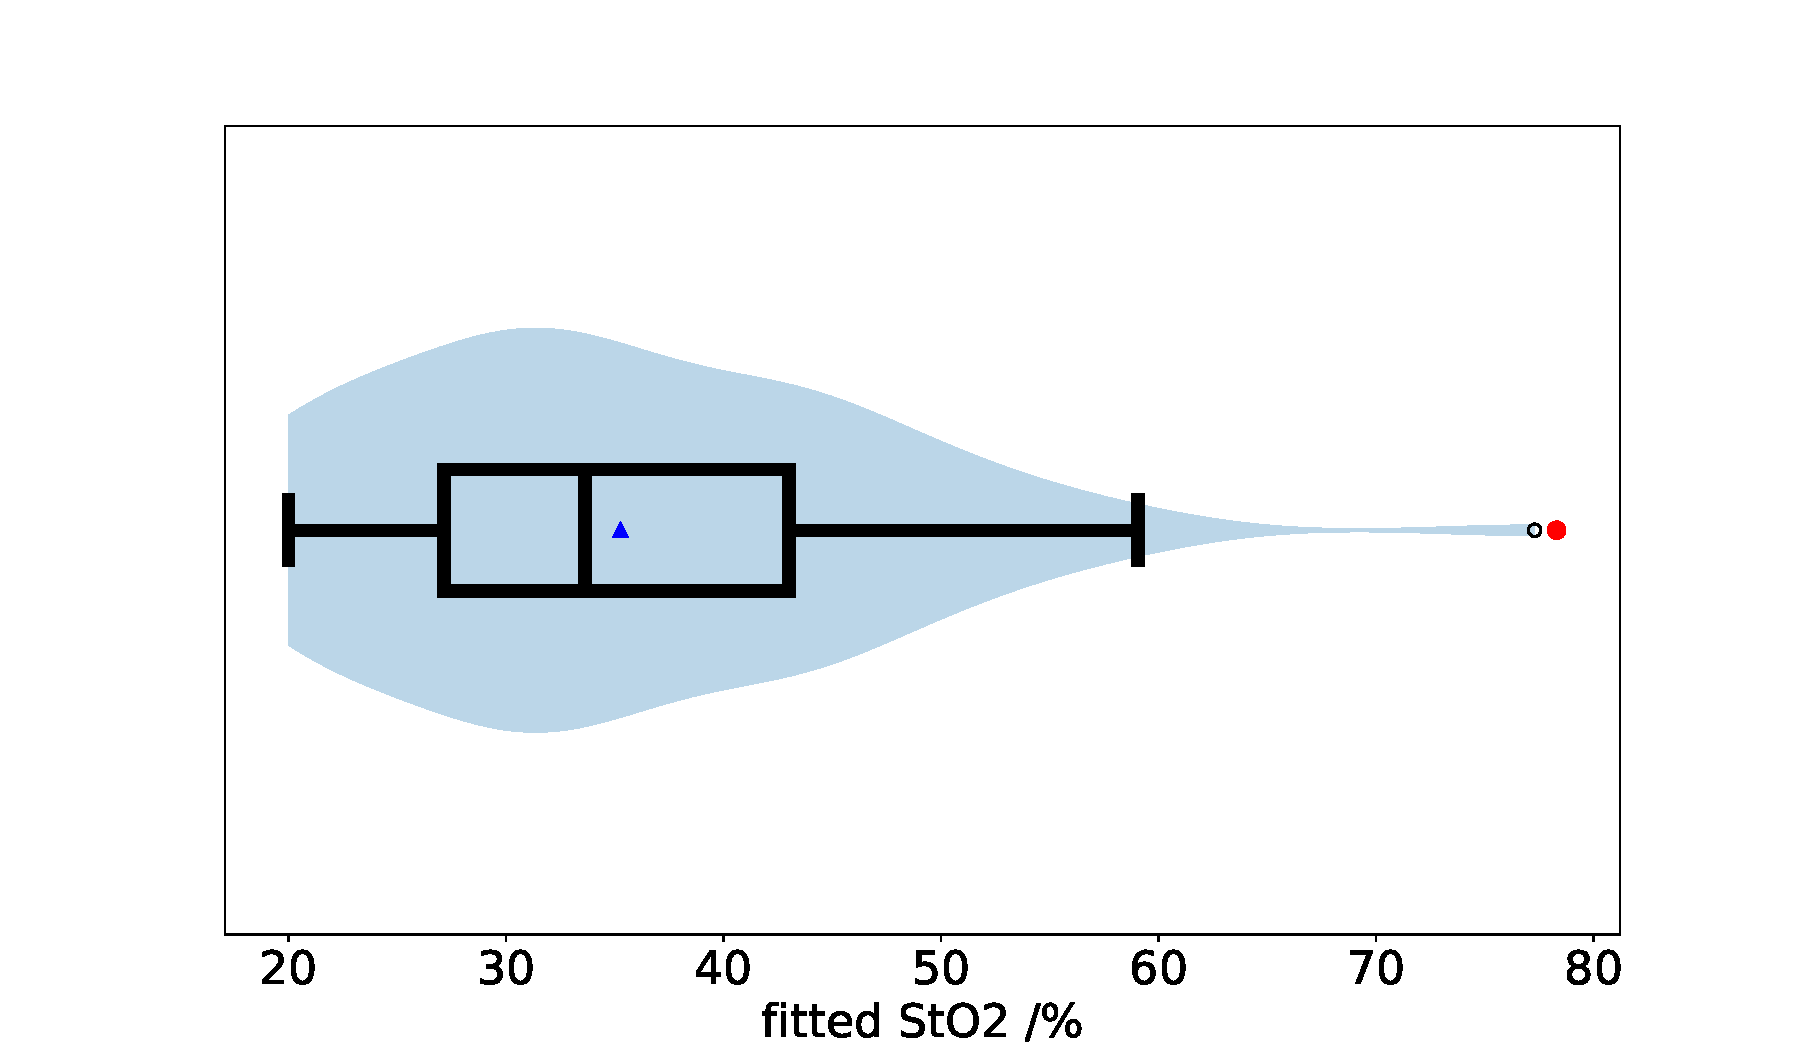
\includegraphics[width=\textwidth]{StO2_boxplot_norm.pdf}
%     %     \caption{}
%     %     \label{fig:egparamStO2NISTnorm}
%     % \end{subfigure}
%     \caption{Examples of the Yudovsky 2009 two layer model fitted to NIST skin total reflectance spectra (\ref{fig:egspectraNIST}) for quantitative (left) or relative (right) data.}
%     \label{fig:NISTfitted}
% \end{figure}

% \begin{figure}[h]
%     \centering
%     \begin{subfigure}{0.8\textwidth}
%         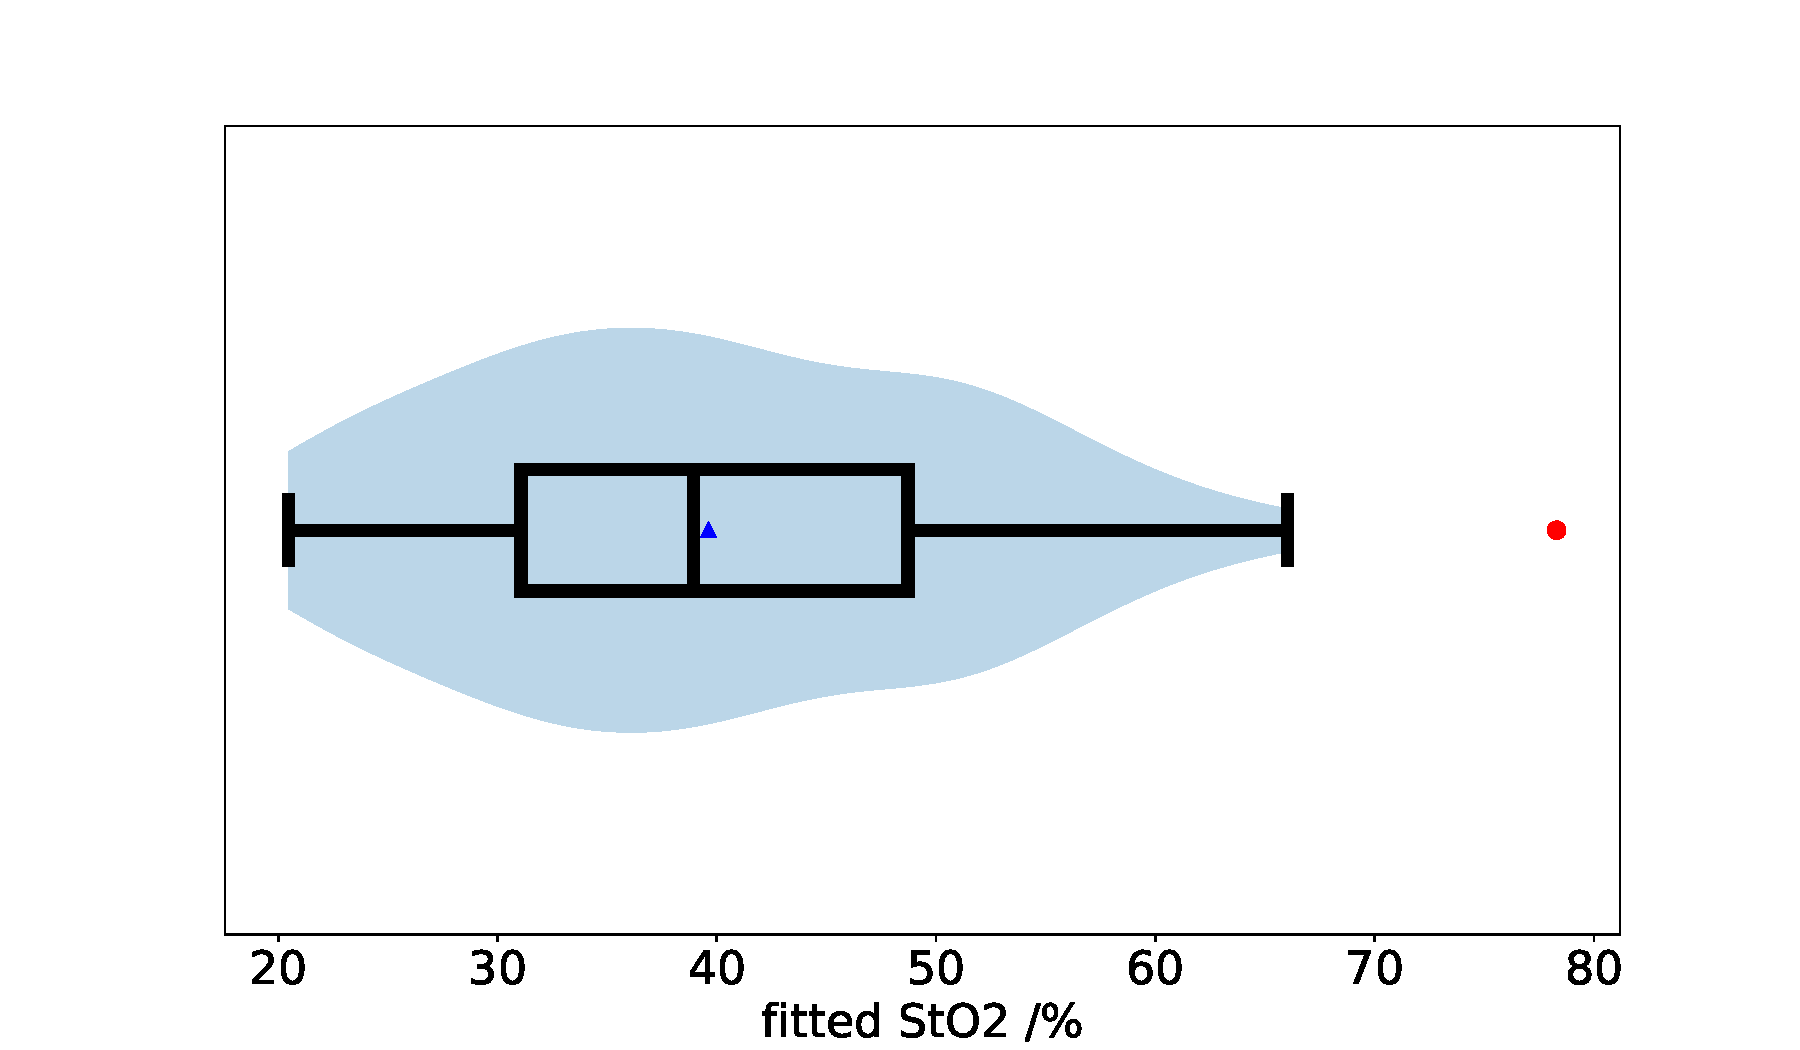
\includegraphics[width=\textwidth]{StO2_boxplot.pdf}
%         \caption{}
%         \label{fig:egparamStO2NIST}
%     \end{subfigure}
%     \begin{subfigure}{0.8\textwidth}
%         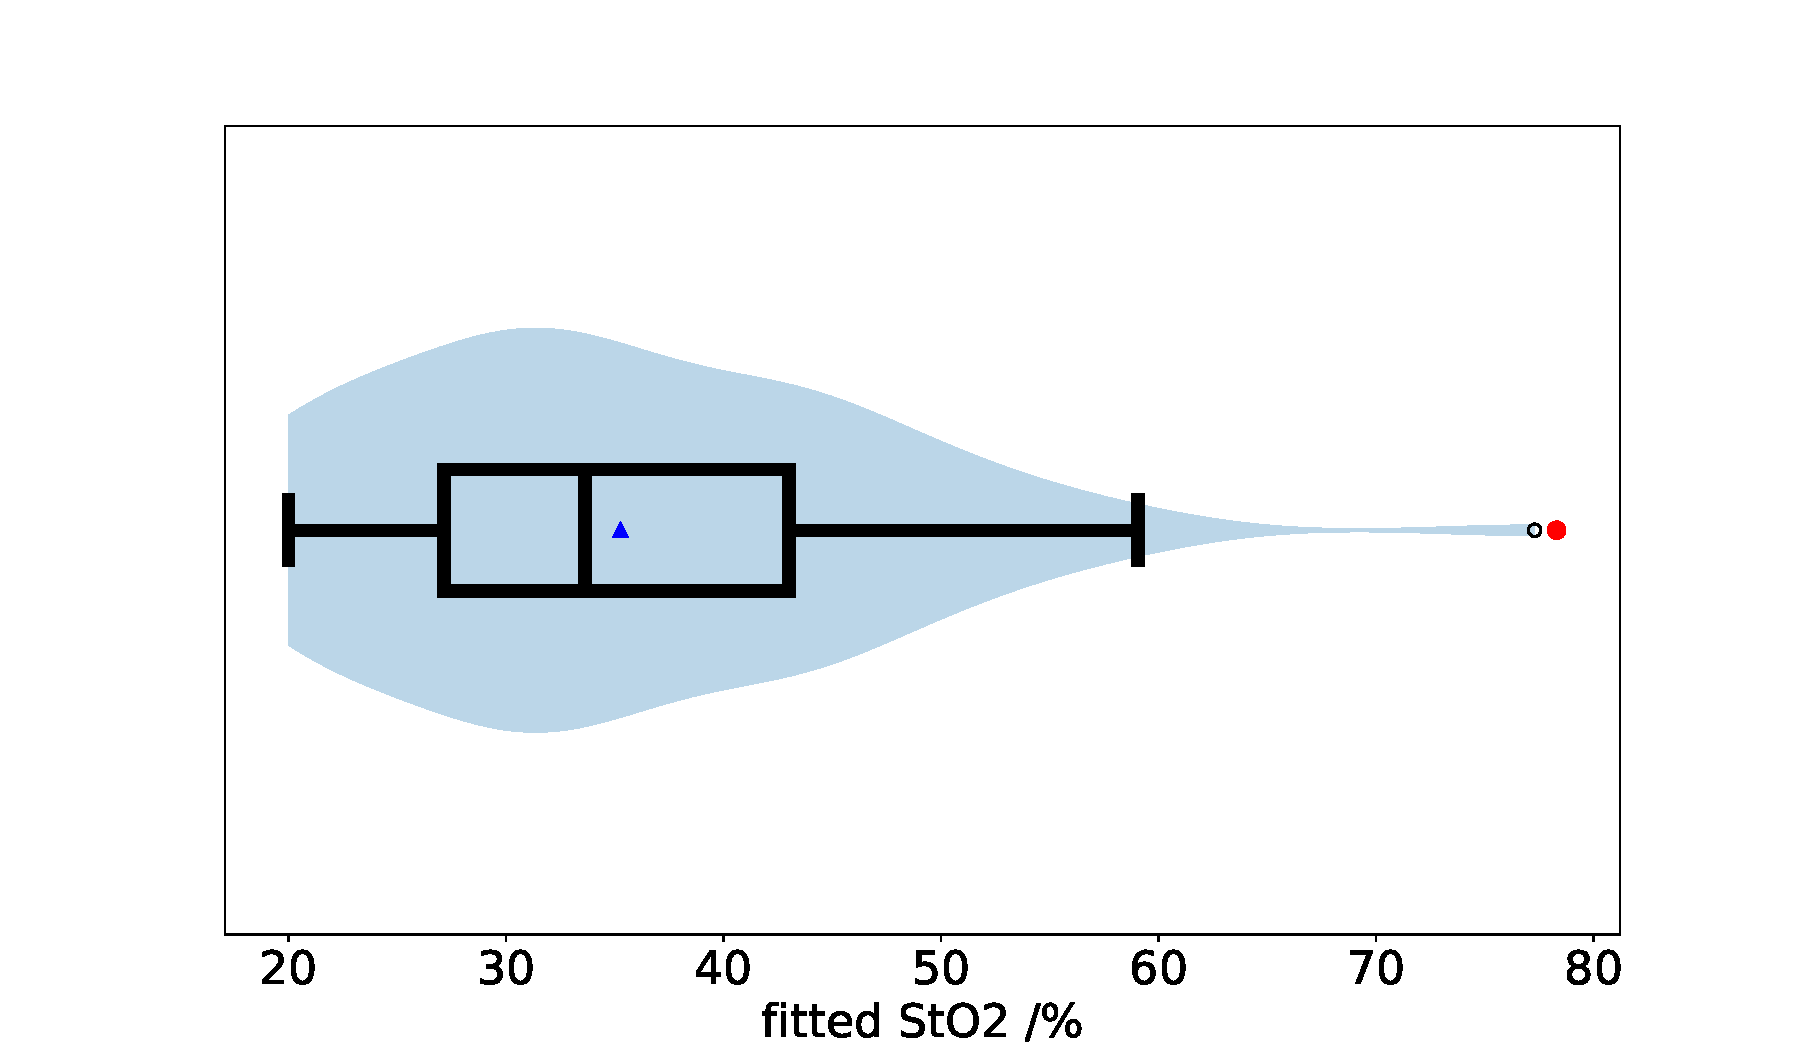
\includegraphics[width=\textwidth]{StO2_boxplot_norm.pdf}
%         \caption{}
%         \label{fig:egparamStO2NISTnorm}
%     \end{subfigure}
%     \caption{Box and violin plots displaying the retrieved $StO_2$ parameters from fitting the Yudovsky 2009 two layer model to the mean NIST skin spectra, where the triangle shows the mean of the fitted $StO_2$ and the circle shows a literature healthy dermis $StO_2$ value \cite{VanManen2021} for quantitative (left) or relative (right) data.}
%     \label{fig:NISTboxplots}
% \end{figure}

\begin{figure}[h]
    \centering
    \begin{subfigure}{0.49\textwidth}
        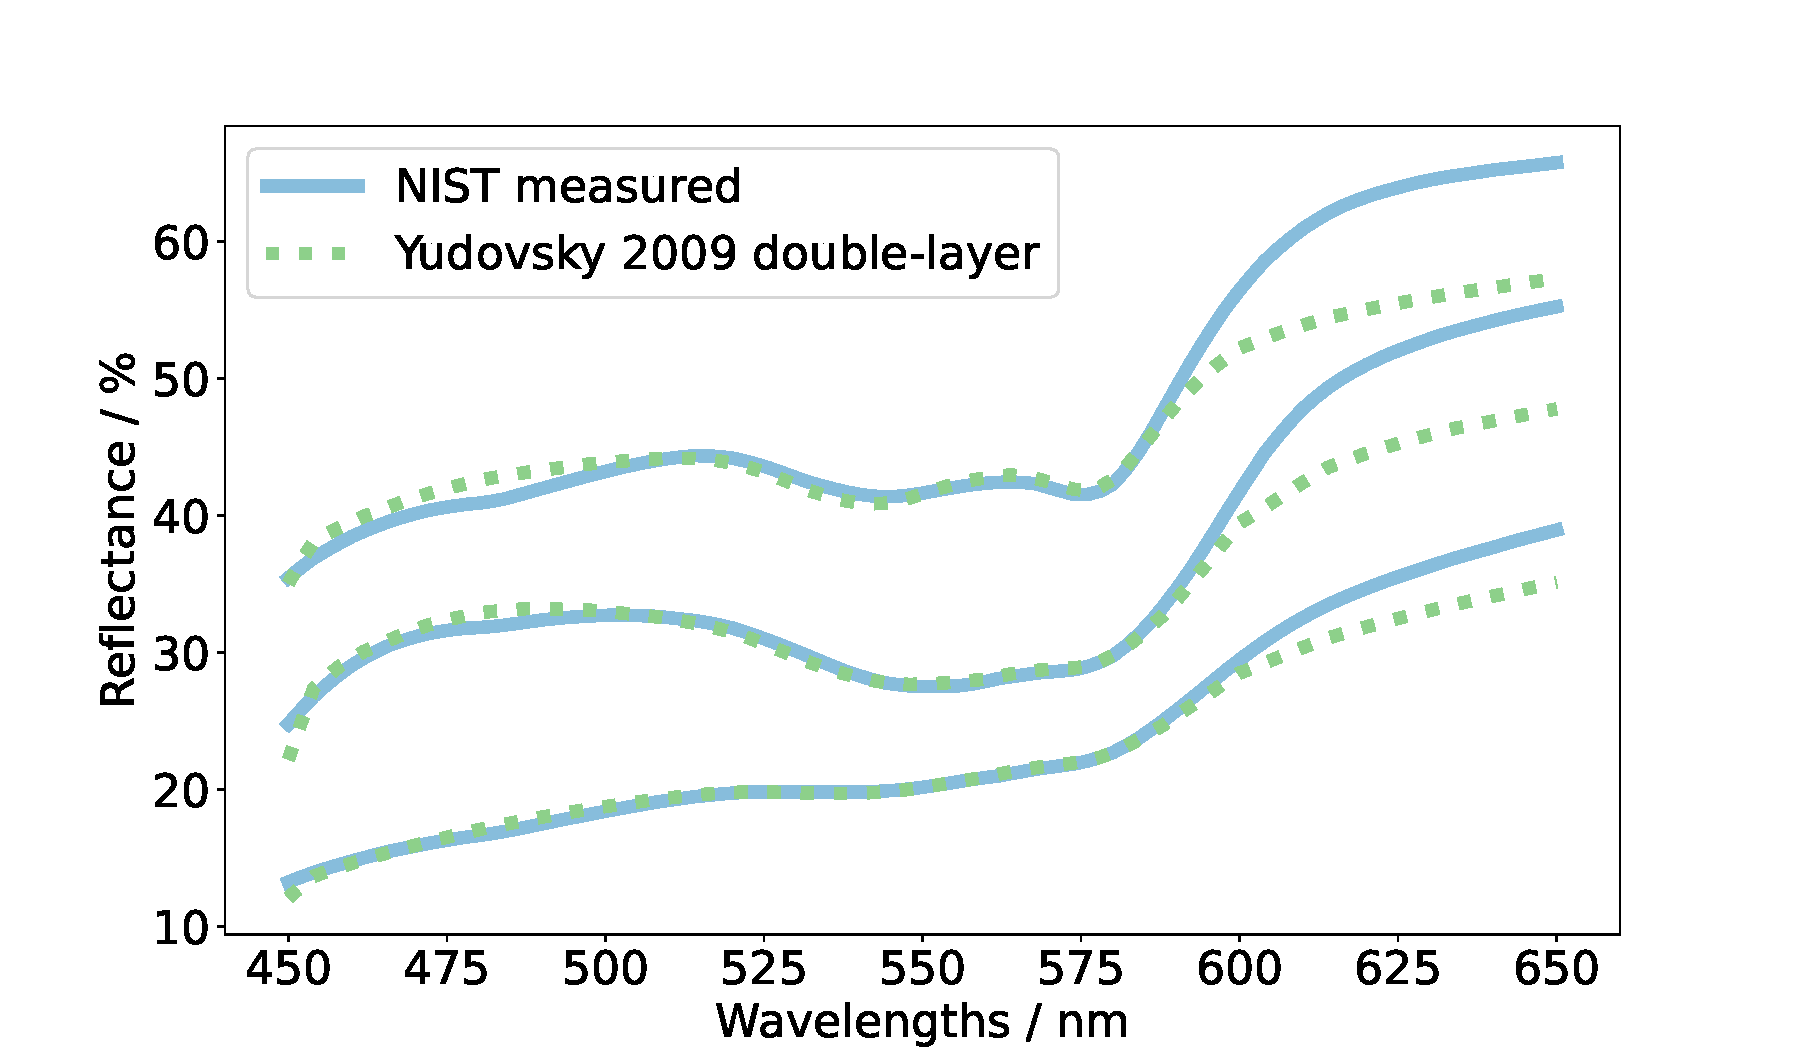
\includegraphics[width=\textwidth]{NIST_Eg.pdf}
        \caption{}
        \label{fig:egspectraNIST}
    \end{subfigure}
    \begin{subfigure}{0.49\textwidth}
        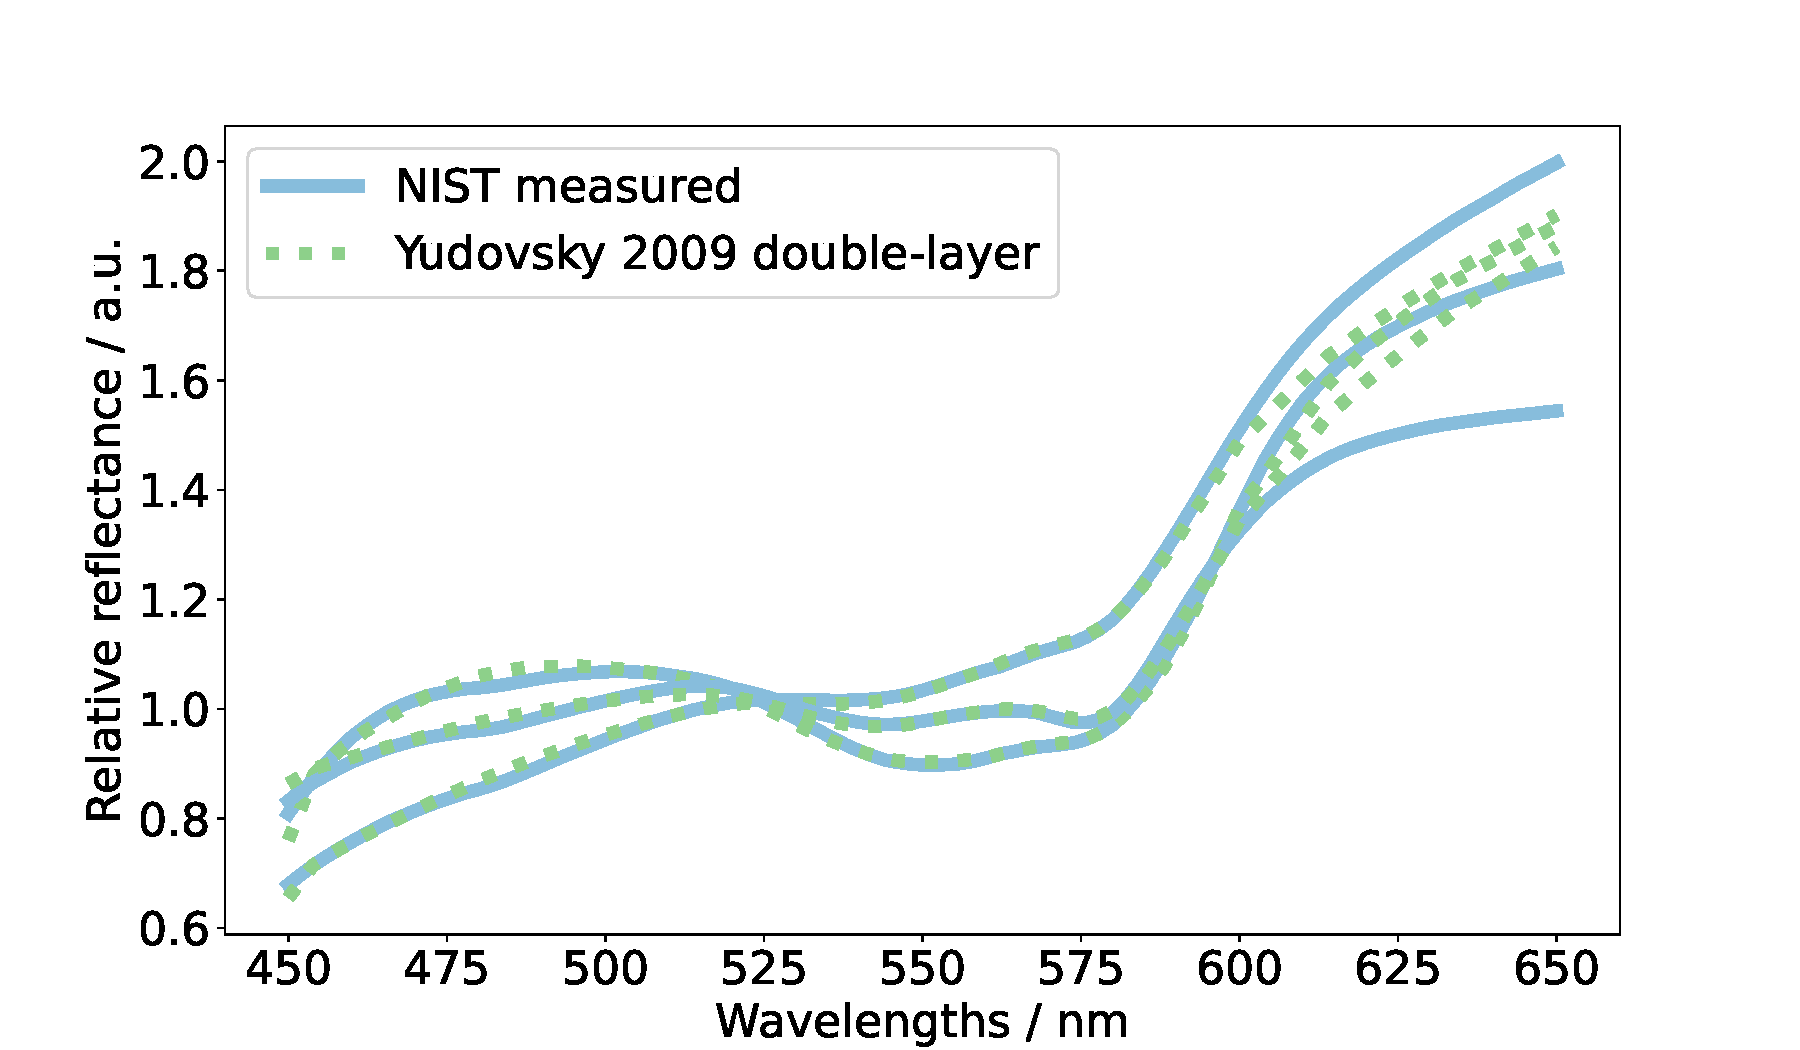
\includegraphics[width=\textwidth]{NIST_Eg_norm.pdf}
        \caption{}
        \label{fig:egspectraNISTnorm}
    \end{subfigure}
    \begin{subfigure}{0.49\textwidth}
        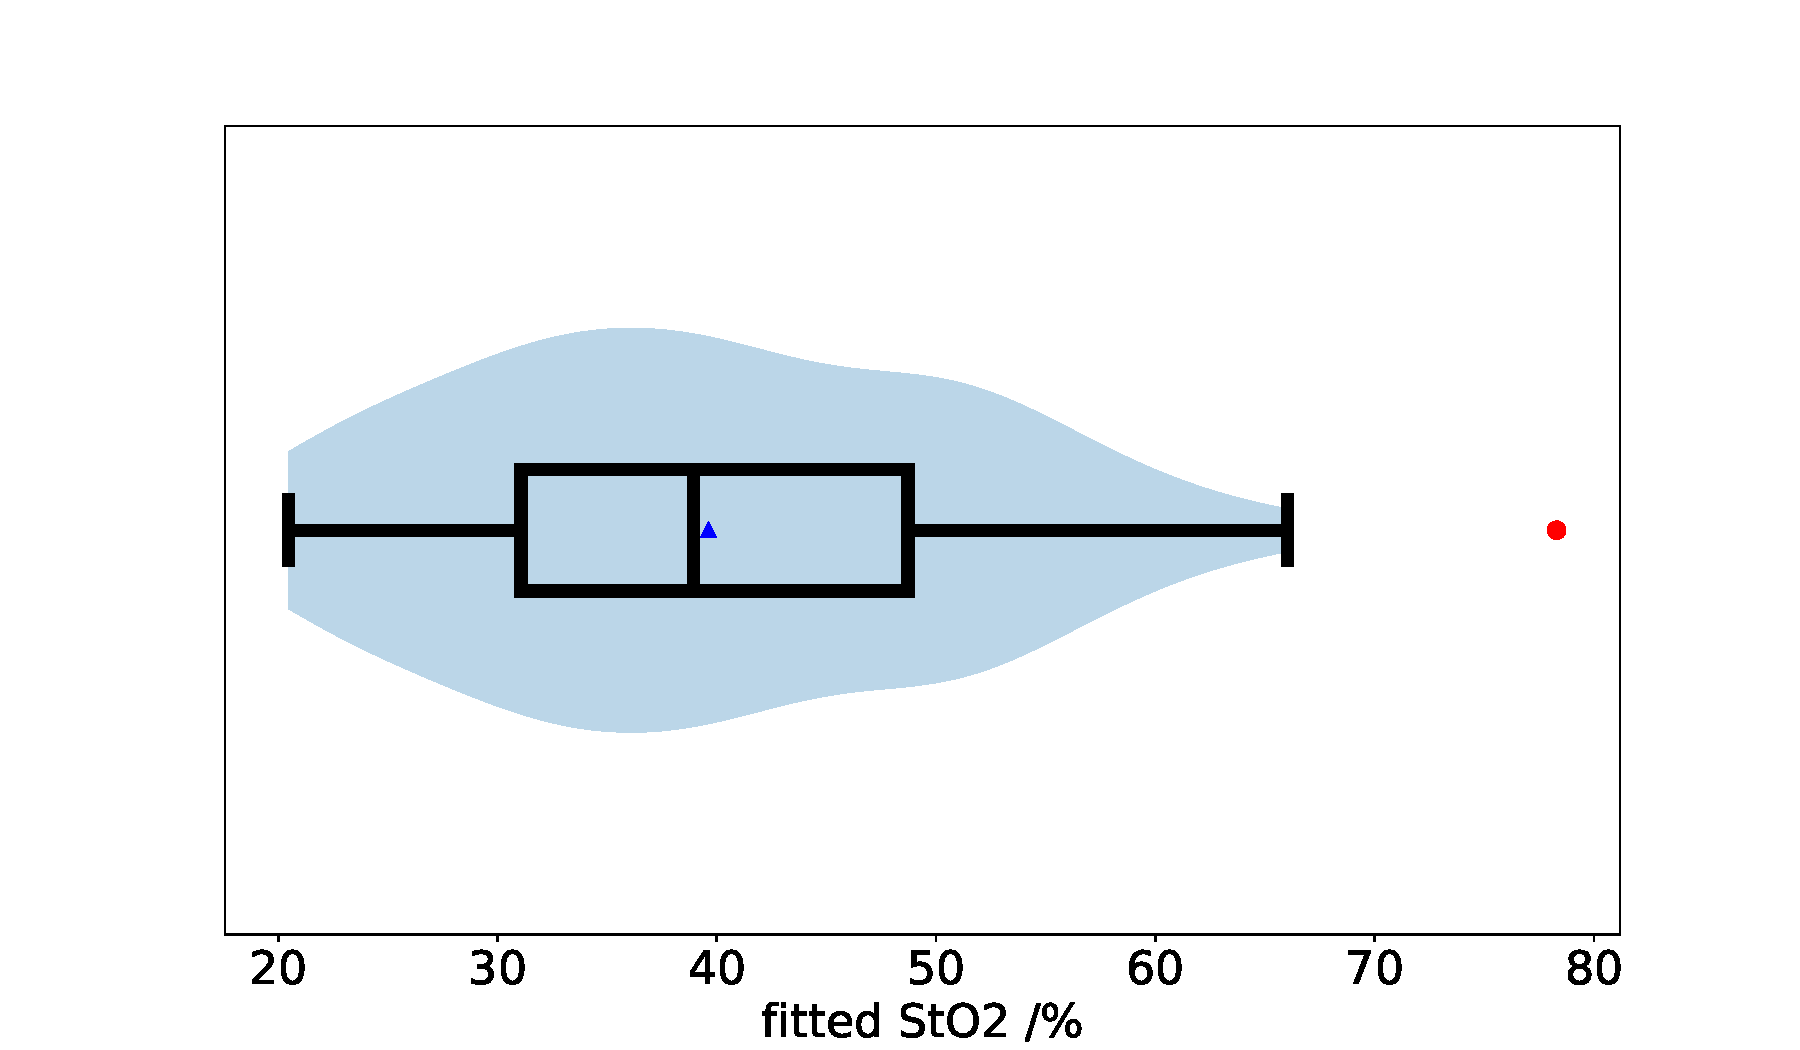
\includegraphics[width=\textwidth]{StO2_boxplot.pdf}
        \caption{}
        \label{fig:egparamStO2NIST}
    \end{subfigure}
    \begin{subfigure}{0.49\textwidth}
        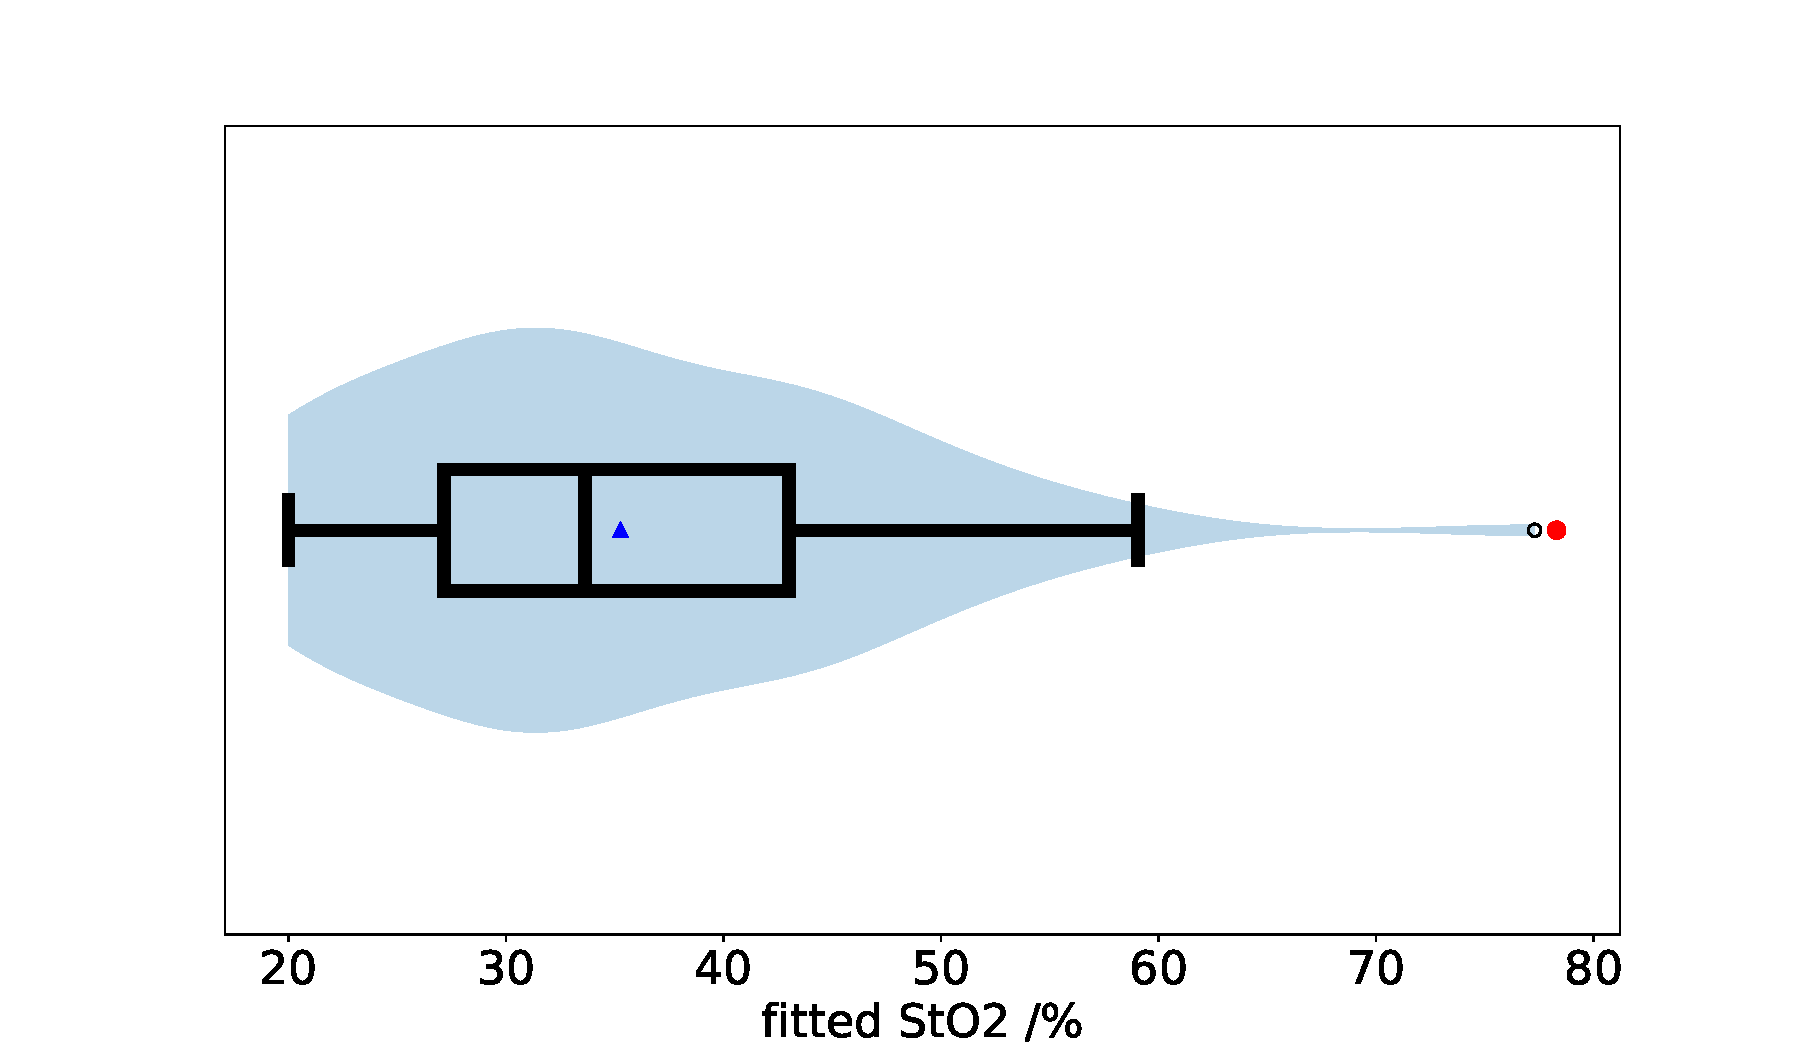
\includegraphics[width=\textwidth]{StO2_boxplot_norm.pdf}
        \caption{}
        \label{fig:egparamStO2NISTnorm}
    \end{subfigure}
    \caption{Top: Examples of the Yudovsky 2009 two layer model fitted to NIST skin total reflectance spectra (\ref{fig:egspectraNIST}) for quantitative (left) or relative (right) data. Bottom: Box and violin plots displaying the retrieved $StO_2$ parameters from fitting the Yudovsky 2009 two layer model to the mean NIST skin spectra, where the triangle shows the mean of the fitted $StO_2$ and the circle shows a literature healthy dermis $StO_2$ value \cite{VanManen2021} for quantitative (left) or relative (right) data.}
    \label{fig:NIST}
\end{figure}
\begin{table}[h]
    \centering
    \caption{The mean and standard deviation for each variable when extracted by fitting Yudovsky 2009 two layer model to the quantitative (Q) or relative (R) NIST skin reflectance dataset, compared to literature parameters for healthy individuals. All presented to 3s.f.}
    \begin{tabular}{|c|ccc|ccc|}
        \hline
        \multirow{2}{*}{Parameter} & \multicolumn{3}{c}{Extracted from NIST dataset} & \multicolumn{3}{|c|}{Literature} \\
        \cline{2-7}
         & Quantitative (Q) & \multirow{2}{*}{Mean} & Standard & \multirow{2}{*}{Mean} & Standard & \multirow{2}{*}{Source} \\
         & or Relative (R) &  & deviation &  & deviation &  \\
        \hline
        \multirow{2}{*}{$StO_2$ (\%)} & Q & 39.6 & 11.1 & \multirow{2}{*}{78.3, 71} & \multirow{2}{*}{12.9, 16} & \cite{VanManen2021} \\ %van manen http://dx.doi.org/10.21037/qims-21-46
        & R & 35.3 & 10.9 & & & \cite{Nishidate2011} \\ %Noninvasive imaging of human skin hemodynamicsusing a digital red-green-blue camera
        \hline
        $f_{blood}$ (\%) & Q & 0.643 & 0.588 & \multirow{2}{*}{1.1} & \multirow{2}{*}{0.4} & \multirow{2}{*}{\cite{Nishidate2011}} \\ %Noninvasive imaging of human skin hemodynamicsusing a digital red-green-blue camera
        & R & 2.72 & 1.82 & & & \\
        \hline
        $f_{mel}$ (\%) & Q & 5.39 & 6.09 & \multirow{2}{*}{4.3} & \multirow{2}{*}{1.2} & \multirow{2}{*}{\cite{Nishidate2011}} \\ %Noninvasive imaging of human skin hemodynamicsusing a digital red-green-blue camera
        & R & 3.61 & 2.95 & & &  \\
        \hline
        $L_1$ ($\mu$m) & Q & 44.3 & 24.3 & \multirow{2}{*}{75.5} & \multirow{2}{*}{N/A} & \multirow{2}{*}{\cite{Lintzeri2022}} \\ %https://www.webofscience.com/wos/woscc/full-record/WOS:000782026000001
        & R & 146 & 15.2 & & &  \\
        \hline
        $a$ (\textrm{$cm^{-1}$}) & Q & 70.0 & 2.91$\times 10^{-8}$ & \multirow{2}{*}{46.0} & \multirow{2}{*}{13.7} & \multirow{2}{*}{\cite{Jacques2013}} \\ %Jacques review
        & R & 47.9 & 13.0 & & &  \\
        \hline
        $b$ (a.u.) & Q & 1.57 & 0.622 & \multirow{2}{*}{1.421} & \multirow{2}{*}{0.517} & \multirow{2}{*}{\cite{Jacques2013}} \\ %Jacques review
        & R & 2.45 & 0.208 & & &  \\
        \hline
    \end{tabular}
    \label{tb:NISTparams}
\end{table}
Examples of the fitted model to some NIST spectra and box plots overlaid with a violin plots for $StO_2$ are shown in Figures \ref{fig:egspectraNIST} and \ref{fig:egspectraNISTnorm} and \ref{fig:egparamStO2NIST} and \ref{fig:egparamStO2NISTnorm} for quantitative and relative data. 
\FloatBarrier

\section{Discussion and Future Work}\label{sec:discussion2}
Whilst the Yudovsky single-layer model has excellent spectral prediction \cite{Bahl2023a}, this quality cannot be replicated by the Yudovsky double-layer model when compared with two-layer Monte Carlo simulations. It is clear that there is significant variability in the performance of the two layer Yudovsky model. This is noted both in the variability of fits to the Monte Carlo spectra and quality of the parameter extraction. The Yudovskly double-layer model spectral prediction is vastly improved when modelling relative data compared to quantitative data as shown by the reduction in $NRMSE$ and the visual fits, however this improvement is not clearly seen in parameter extraction from the Monte Carlo data. The most robust parameter extraction from this model is for $StO_2$. Leveraging this, the weaknesses of this model can be shown to be in regions of high $L_1$, high $f_{mel}$, and low $f_{blood}$. This follows intuition that in regions where the melanin impact in the epidermis is significant, it "masks" a low haemoglobin impact from the dermis. For this reason, this model should be used with caution as it has limited use in the regions of failure identified.

Whilst this model appears to fit well to NIST skin experimental data when using a least-squares fitting routine, the parameters it returns are largely very different to previous literature values for healthy individuals. The dermal layer is modelled identically to the single layer model which has been shown to perform well with well-characterised experimental data \cite{Bahl2023a}, suggesting that there are interactions between layers or biological components that are not appropriately accounted for or that the optical properties of these tissue types are not well characterised. 

In conclusion, this work demonstrates that the double-layer Yudovsky model does not always perform with the same quality as the single-layer model. Combining this with the parameters extracted from the NIST dataset which do not correspond to other literature values and the failure regions depicted, demonstrates that this model should be used with caution. 

This work should be viewed in light of it's limitations which include the lack of ground-truth parameters for the NIST skin dataset. It is challenging to obtain reliable ground-truth values for any in-vivo skin measurements so the results from this model's parameter extraction cannot be quantitatively evaluated easily. 

Future work should include investigation of the epidermis, similarly to investigation of the single-layer models with the dermis, and interaction between the layers to improve this model. This model could also be tested with layered tissue-mimicking optical phantoms with known ground truth parameters to allow full quantitative evaluation of the model performance with experimental data. 
%After improvement of the performance with experimental data, this model could be adapted for use with hyperspectral imaging cameras which may not have as densely sampled spectra, as these have been shown to be likely methods of obtaining these diffuse reflectance spectra intra-operatively \cite{Clancy2020}. 

In the context of this thesis, this model is investigated for use within the brain. Here some of the layered structures may not have absorbing chromophores as powerful as melanin, e.g. Pia Mater, so it is more likely the parameters of these tissues will lie within the successful region of parameter space where both layers can be characterised well. For this reason this model is investigated further in Chapter \ref{chap:HSImodel}, however only low absorbing layers are considered for layer 1. 

% \bibliography{Paper3}
% \bibliographystyle{spiejour}
% \end{document}